\documentclass[11pt,a4paper]{article}

% Packages
\usepackage[utf8]{inputenc}
\usepackage[T1]{fontenc}
% Typography: URW Palatino (Palladio) text + Pazo math + Inconsolata mono.
% This is the same font stack used by the Qwen technical reports.
\usepackage{mathpazo}
\usepackage[scaled=0.95]{inconsolata}
\usepackage{microtype}
\usepackage{amsmath,amssymb,amsfonts}
\usepackage{graphicx}
\usepackage[numbers,sort&compress]{natbib}
\usepackage{booktabs}
\usepackage{tabularx}
\usepackage{multirow}
\usepackage{xcolor}
\usepackage{fancyhdr}
\usepackage{enumitem}
\usepackage{tcolorbox}
\usepackage{tikz}
\usetikzlibrary{arrows.meta, positioning, fit, backgrounds, calc, shapes.geometric}
\usepackage[margin=1in]{geometry}
\usepackage[hidelinks]{hyperref}

% Resolve assets/figures whether compiled from the repo root or this folder.
\graphicspath{{./}{figures/}{../../template/}{template/}}

% Brand header (logo + wordmark on the left, date on the right)
\definecolor{gaussiadark}{HTML}{323030}
\definecolor{gaussiaccent}{HTML}{C15A35}
\definecolor{gaussiasoft}{HTML}{F3ECE7}
\definecolor{gaussiablue}{HTML}{3A6EA5}
\newcommand{\paperdate}{July 24, 2026}
\newcommand{\papersurl}{https://www.gaussia.ai/papers}
\newcommand{\repourl}{https://github.com/gaussia-labs/papers}
\newcommand{\hfurl}{https://huggingface.co/gaussia-labs}
% Header logo (no link, just branding)
\newcommand{\gaussialogo}{%
  \raisebox{-0.28\height}{
\includegraphics[height=14pt]{logo}}%
  \hspace{5pt}\textcolor{gaussiadark}{\textbf{\large Gaussia}}%
}
% Clickable links shown under the title, Qwen-report style
\newcommand{\paperlinks}{%
  \begin{center}
    \href{\repourl}{%
      \raisebox{-0.22\height}{
\includegraphics[height=11pt]{github}}%
      \hspace{4pt}\texttt{github.com/gaussia-labs/papers}}\\[4pt]
    \href{\papersurl}{%
      \raisebox{-0.26\height}{
\includegraphics[height=11pt]{logo}}%
      \hspace{4pt}\texttt{gaussia.ai/papers}}\\[4pt]
    \href{\hfurl}{%
      \raisebox{-0.26\height}{
\includegraphics[height=12pt]{hf-logo}}%
      \hspace{4pt}\texttt{huggingface.co/gaussia-labs}}
  \end{center}%
}

\providecommand{\keywords}[1]{%
  \vspace{0.5em}%
  \noindent\textbf{Keywords: }#1%
}

\setlength{\headheight}{18pt}
\pagestyle{fancy}
\fancyhf{}
\lhead{\gaussialogo}
\rhead{\textcolor{gaussiadark}{\paperdate}}
\renewcommand{\headrulewidth}{0.6pt}
\rfoot{\thepage}

% ---- Shared callout box ----------------------------------------------------
\newtcolorbox{callout}[1][]{
  colback=gaussiasoft, colframe=gaussiaccent,
  boxrule=0.6pt, arc=2pt, left=6pt, right=6pt, top=5pt, bottom=5pt,
  fonttitle=\bfseries, #1
}

% ---- Shared TikZ styles ----------------------------------------------------
\tikzset{
  box/.style={draw=gaussiadark, rounded corners=3pt, thick, align=center,
              font=\small, inner sep=6pt, fill=white},
  accentbox/.style={box, draw=gaussiaccent, fill=gaussiasoft},
  bluebox/.style={box, draw=gaussiablue, fill=blue!5},
  smallbox/.style={box, font=\footnotesize, inner sep=4pt},
  flow/.style={-{Stealth[length=2.5mm]}, thick, draw=gaussiadark},
  flowa/.style={-{Stealth[length=2.5mm]}, thick, draw=gaussiaccent},
  lbl/.style={font=\footnotesize\itshape, text=gaussiadark},
}

% Ragged-right flexible column: avoids stretched spacing in narrow table cells.
\newcolumntype{Y}{>{\raggedright\arraybackslash}X}

% ---- Coverage symbols for the requirements matrix ---------------------------
\newcommand{\cfull}{\tikz[baseline=-0.5ex]\fill[gaussiaccent](0,0)circle(0.85ex);}
\newcommand{\cpart}{\tikz[baseline=-0.5ex]{%
  \draw[gaussiaccent, thick](0,0)circle(0.85ex);
  \fill[gaussiaccent](0,0.85ex) arc(90:270:0.85ex)--cycle;}}
\newcommand{\cnone}{\tikz[baseline=-0.5ex]\draw[gaussiadark!45, thick](0,0)circle(0.85ex);}

% Metadata
\title{\textbf{Boltzmann Brain: A Versioned, Distributable, and\\
Model-Agnostic Knowledge Architecture}}
\author{
  Alex Fiorenza \\
  \texttt{alexfiorenza2012@gmail.com} \\
  Gaussia
}
\date{}

\begin{document}

\maketitle
\thispagestyle{fancy}

% Repository and website links, shown under the title
\paperlinks

% The abstract is REQUIRED for every Gaussia paper. Do not remove it.
\begin{abstract}
Knowledge produced with large language models (LLMs) tends to become locked
inside a single provider, agent, or vector store, where it is hard to audit,
reindex, version, or move. We propose \textbf{Boltzmann Brain}, a portable
knowledge architecture built on one principle: the brain conserves, validates,
and retrieves knowledge, while an external and interchangeable LLM processes,
contextualizes, and uses it. The brain never embeds a model of its own.
Knowledge is stored as typed, content-addressed blocks organized into five
memory modules (canonical, episodic, semantic, procedural, and provenance),
inspired by complementary learning systems and hippocampal indexing rather
than by literal brain-to-database mappings. Each module bundles its blocks, a
Merkle DAG that pins the exact composition of a version, and the indices needed
to query it. We separate three levels of hashes, one for block identity, one
for the Merkle root of a snapshot, and one for the OCI digest of a distributed
blob, and show how packaging each module as a separate OCI Artifact yields
selective installation and incremental updates. Interaction happens through the
\emph{Boltzmann Protocol}: during ingestion and query the LLM proposes candidate
blocks and consumes Evidence Bundles, while the protocol governs what is
committed and returns only verified evidence, never prose. Because the brain is
portable data addressed by a protocol rather than a deployable service, the same
snapshot can be read and extended by any conforming client. Canonical blocks are
the root of evidence: they record what was observed, not what is true, and every
derived interpretation cites them through provenance. Because wrong knowledge
must be removable without punching holes in the current snapshot, we specify how
non-episodic modules drop blocks, rebuild their Merkle DAGs, and cascade through
provenance, with a privileged cascade when the dropped block is canonical, and
with redaction reserved for destroying retained bytes. Beyond the architecture,
this version fixes the wire formats an independent implementation needs in order
to interoperate: the block envelope and its canonical serialization, the Merkle
construction and its layout identifier, the composition and snapshot documents,
the OCI media types and annotations, the ingestion and query contracts, and a
conformance kit of golden vectors. What remains open is authenticity: the
protocol establishes that an artifact is intact, not who produced it, and it
defines no reconciliation for two brains that diverged.
\end{abstract}

\keywords{knowledge representation, retrieval-augmented generation, content
addressing, Merkle DAG, OCI Artifacts, memory systems, LLM agents}

% ===========================================================================
\section{Introduction}
\label{sec:intro}

Large language models have made it cheap to \emph{produce} knowledge (notes,
summaries, extracted facts, procedures), but expensive to \emph{own} it. In
practice, the knowledge a user accumulates while working with an LLM tends to
be captured in a form dictated by whichever provider, agent framework, or
vector database happens to be in use. Embeddings are computed with a specific
model, chunks are shaped by a specific pipeline, and the resulting store is
rarely portable, verifiable, or re-interpretable. When the model changes, the
provider changes, or the indexing strategy changes, the knowledge is often
effectively lost, or must be rebuilt from scratch.

This paper argues that knowledge should be a \emph{first-class, portable
artifact} that outlives any particular model or vendor. We present
\textbf{Boltzmann Brain}, an architecture whose sole responsibility is to
conserve information, organize it into memories with distinct purposes,
maintain verifiable versions, and retrieve relevant evidence. Crucially, the
brain contains no language model of its own. It integrates with whatever LLM
the user chooses, which interprets sources during ingestion and contextualizes
results during query. The design is captured by a single guiding idea:

\begin{callout}
\emph{The brain conserves, validates, and retrieves knowledge. An external LLM
processes, contextualizes, and uses it.}
\end{callout}

\paragraph{The responsibility boundary.}
The brain does not write the final answer. It returns knowledge blocks and
evidence; an agent, interface, or downstream application decides how to
contextualize them (Figure~\ref{fig:separation}). This boundary is what keeps
the architecture independent of any provider: the Boltzmann Protocol governs
structure, identity, validation, and distribution, while the semantic work
(reading, extracting concepts, recognizing episodes, proposing procedures, and
phrasing answers) is delegated to an interchangeable external model.

\paragraph{Contributions.}
This work makes the following contributions:
\begin{enumerate}[leftmargin=1.4em]
  \item A set of design principles and problems (Section~\ref{sec:principles})
  for portable, verifiable, model-agnostic knowledge, and an argument for why
  six requirements that existing work satisfies separately must hold over a
  single artifact (Section~\ref{sec:related}).
  \item A mapping from biological memory principles and classic systems
  structures to concrete architectural decisions (Section~\ref{sec:inspiration}).
  \item A five-module memory model (canonical, episodic, semantic,
  procedural, and provenance; Section~\ref{sec:modules}) that treats the
  canonical module as the root of observed evidence, together with an internal
  module anatomy of content-addressed blocks, Merkle DAGs, and indices
  (Section~\ref{sec:anatomy}).
  \item A distribution model based on OCI Artifacts that enables selective
  installation and incremental updates (Section~\ref{sec:distribution}), and a
  model-agnostic protocol with explicit ingestion and query contracts
  (Sections~\ref{sec:protocol}--\ref{sec:query}).
  \item A treatment of how knowledge leaves a brain
  (Section~\ref{sec:forgetting}): drop with Merkle rebuild and provenance
  cascade for non-episodic modules, a privileged cascade when canonical evidence
  is excluded, supersession for episodic memory, pruning of unreachable blocks,
  and redaction when retained bytes must be destroyed.
  \item A normative encoding for all of the above: the block envelope and its
  canonical serialization (Section~\ref{sec:serialization}), the Merkle
  construction and its layout identifier (Section~\ref{sec:merkle}), the
  composition and snapshot documents (Sections~\ref{sec:composition-doc}
  and~\ref{sec:snapshot}), the schema-versioning rules that let old clients read
  new brains (Section~\ref{sec:schema-versioning}), and a conformance kit of
  golden vectors (Section~\ref{sec:conformance}).
\end{enumerate}

\paragraph{Scope of this version.}
This document fixes both an architecture and the interoperability surface that
follows from it. Everything two independent implementations must agree on to
exchange a brain is normative here: the block envelope, the canonical
serialization, the Merkle construction, the composition and snapshot documents,
the distribution encoding, and the ingestion and query contracts
(Section~\ref{sec:conformance} states how an implementation demonstrates
agreement). What stays deliberately open is what an implementation may choose
without breaking exchange: consolidation and contradiction-detection
strategies, ranking and fusion, index engines, and pack sizing. Two questions
remain open in the normative surface itself, and Section~\ref{sec:conclusion}
states them as such: authenticity of authorship, and reconciliation of diverged
brains.

\paragraph{Notational conventions.}
The key words \textbf{MUST}, \textbf{MUST NOT}, \textbf{SHOULD}, and
\textbf{MAY} are used as defined in RFC 2119~\cite{rfc2119}. A
\emph{conforming implementation} is one that satisfies every MUST in this
document for the roles it claims (Section~\ref{sec:conformance}). Documents are
shown as JSON for readability; the bytes that are hashed are always the
canonical serialization of Section~\ref{sec:serialization}, never the
pretty-printed form.

\begin{figure}[t]
\centering
\begin{tikzpicture}[node distance=10mm]
  \node[accentbox, text width=4.4cm] (brain) {\textbf{Boltzmann Brain}\\[2pt]
    \footnotesize conserves $\cdot$ validates $\cdot$ retrieves\\[3pt]
    \scriptsize typed blocks, Merkle DAGs,\\ indices, provenance};
  \node[bluebox, right=32mm of brain, text width=4.4cm] (llm) {\textbf{External LLM}\\[2pt]
    \footnotesize processes $\cdot$ contextualizes $\cdot$ uses\\[3pt]
    \scriptsize interprets sources,\\ phrases the final answer};
  \draw[flowa] ([yshift=4pt]brain.east) -- node[lbl, above]{Evidence Bundle}
    ([yshift=4pt]llm.west);
  \draw[flow] ([yshift=-4pt]llm.west) -- node[lbl, below]{candidate blocks}
    ([yshift=-4pt]brain.east);
  \node[smallbox, below=9mm of brain, text width=4.4cm, draw=gaussiadark]
    (store) {\footnotesize canonical $\cdot$ episodic $\cdot$ semantic\\
    procedural $\cdot$ provenance};
  \draw[flow] (brain) -- (store);
  \node[smallbox, below=9mm of llm, text width=4.4cm, draw=gaussiablue]
    (user) {\footnotesize user / agent / application};
  \draw[flow] (llm) -- (user);
\end{tikzpicture}
\caption{Separation of responsibilities. The brain owns knowledge, identity,
and verification; the external LLM owns interpretation and phrasing. The two
communicate through a stable contract: the LLM sends candidate blocks during
ingestion and receives Evidence Bundles during query.}
\label{fig:separation}
\end{figure}

% ===========================================================================
\section{Design Principles and Problems}
\label{sec:principles}

\subsection{Problems this architecture addresses}

Boltzmann Brain is designed to address a cluster of related failures in how
LLM-era knowledge is currently stored and consumed:

\begin{itemize}[leftmargin=1.4em]
  \item Preventing knowledge from being trapped inside a particular provider,
  agent, or vector database.
  \item Maintaining a source of evidence that allows knowledge to be
  reindexed and reinterpreted as models and methods evolve.
  \item Distinguishing concrete experiences, general facts, and procedures,
  rather than collapsing everything into undifferentiated chunks.
  \item Updating knowledge without losing history, provenance, or
  reproducibility.
  \item Removing knowledge that is obsolete, costly, or legally untenable,
  without silently compromising verifiability.
  \item Distributing a complete brain or only selected modules.
  \item Allowing interchangeable external LLMs to query and contribute
  knowledge through a stable contract.
\end{itemize}

\subsection{Guiding principles}

Eight principles follow from these problems and constrain every subsequent
design decision:

\begin{enumerate}[leftmargin=1.6em]
  \item Knowledge lives in blocks; indices are not the source of truth.
  \item Original evidence is preserved by default; interpretations may change.
  Dropping a canonical block is allowed only under explicit policy, and it
  forfeits re-derivation from that source.
  \item Every version must be identifiable, verifiable, and reconstructible.
  \item Modules must be distributable and installable selectively.
  \item The protocol must not embed an LLM of its own nor depend on a specific
  provider.
  \item Specialized structures compose; no single index answers every query.
  \item Queries are declarative and index-agnostic: callers ask for knowledge,
  and the selection and combination of indices is left to the implementation.
  \item Forgetting is explicit and auditable: non-episodic modules support drop
  with Merkle rebuild and provenance cascade; dropping canonical evidence is
  privileged and always cascades; content may be redacted under policy, but
  never silently.
\end{enumerate}

These principles are intentionally conservative. They privilege durability and
auditability over convenience, and they treat the LLM as a powerful but
replaceable interpreter rather than as the system of record.

% ===========================================================================
\section{Inspirations}
\label{sec:inspiration}

\subsection{Biology of memory}

The architecture takes \emph{general principles} from neuroscience, not
literal equivalences between brain regions and databases. The scientific
literature describes multiple memory systems and an interaction among fast
learning, stable knowledge, consolidation, associative recall, and adaptive
forgetting~\cite{kumaran2016cls, goode2018engram, yassa2011pattern,
knierim2016tracking, rebola2017pattern, nader2009reconsolidation,
redondo2011tagging, ryan2022forgetting}. Figure~\ref{fig:biology} summarizes
the translation from biological principles to architectural decisions.

Complementary learning systems (CLS) theory distinguishes a fast,
hippocampus-associated mechanism from slower, integrative cortical
learning~\cite{kumaran2016cls}. For Boltzmann Brain this suggests separating
the \emph{capture of episodes} from \emph{semantic consolidation}. The
hippocampal indexing theory further motivates a distinction between the index
that reactivates a memory and the distributed content of that
memory~\cite{goode2018engram}, a distinction we mirror in our separation of
indices from knowledge blocks. Pattern separation inspires deduplication, identity
resolution, and contradiction detection; pattern completion inspires
recovering a full memory from a partial query through hybrid
search~\cite{yassa2011pattern, knierim2016tracking, rebola2017pattern}.
Finally, reconsolidation suggests that retrieving knowledge can open a
controlled revision~\cite{nader2009reconsolidation, redondo2011tagging}, while
work on pruning and active forgetting suggests that removing what is not
reinforced is a regulated process rather than a failure, and that accessibility
can be reduced without destroying the underlying
evidence~\cite{paolicelli2011pruning, davis2017forgetting, ryan2022forgetting}.
Section~\ref{sec:forgetting} develops this last point into concrete retention
and erasure mechanisms.

\begin{figure}[t]
\centering
\begin{tikzpicture}[node distance=6mm and 22mm]
  \node[bluebox, text width=4.2cm] (b1) {\footnotesize Fast vs.\ slow\\ learning (CLS)};
  \node[bluebox, below=of b1, text width=4.2cm] (b2) {\footnotesize Hippocampal\\ indexing};
  \node[bluebox, below=of b2, text width=4.2cm] (b3) {\footnotesize Pattern separation\\ \& completion};
  \node[bluebox, below=of b3, text width=4.2cm] (b4) {\footnotesize Reconsolidation};
  \node[bluebox, below=of b4, text width=4.2cm] (b5) {\footnotesize Synaptic pruning \&\\ active forgetting};

  \node[accentbox, right=of b1, text width=4.6cm] (a1) {\footnotesize Split episodic capture\\ from semantic consolidation};
  \node[accentbox, right=of b2, text width=4.6cm] (a2) {\footnotesize Indices separate from\\ knowledge blocks};
  \node[accentbox, right=of b3, text width=4.6cm] (a3) {\footnotesize Dedup, identity resolution,\\ hybrid retrieval};
  \node[accentbox, right=of b4, text width=4.6cm] (a4) {\footnotesize Controlled revision;\\ supersede without deleting};
  \node[accentbox, right=of b5, text width=4.6cm] (a5) {\footnotesize Drop with Merkle rebuild;\\ prune unreachable blocks};

  \draw[flowa] (b1) -- (a1);
  \draw[flowa] (b2) -- (a2);
  \draw[flowa] (b3) -- (a3);
  \draw[flowa] (b4) -- (a4);
  \draw[flowa] (b5) -- (a5);
  \node[lbl, above=1mm of b1] {Biological principle};
  \node[lbl, above=1mm of a1] {Architectural decision};
\end{tikzpicture}
\caption{Translation of biological memory principles into architectural
decisions. The mapping is by analogy, not by literal correspondence between
brain regions and system components.}
\label{fig:biology}
\end{figure}

\subsection{Systems structures}

Alongside biology, the architecture reuses well-understood systems structures.
Table~\ref{tab:systems} lists each one and its contribution.

\begin{table}[htb]
\centering
\caption{Systems structures and their contribution to Boltzmann Brain.}
\label{tab:systems}
\begin{tabularx}{\textwidth}{lX}
\toprule
\textbf{Concept} & \textbf{Contribution to Boltzmann Brain} \\
\midrule
Content addressing        & The identity of a block derives from its content. \\
Merkle DAG                & A root identifies the exact composition of a module. \\
B\textsuperscript{+} tree & Exact lookup, hierarchies, and ordered range scans. \\
Inverted index            & Lexical search over words and terms. \\
Vector index              & Approximate retrieval by semantic similarity. \\
Graph                     & Explicit relations, provenance, associative expansion. \\
Mark-and-sweep collection & Reclaiming blocks unreachable from a retained root. \\
OCI Artifact              & Interoperable packaging and distribution of modules. \\
Skill / MCP / CLI / API   & Contract for an external LLM to query and ingest. \\
\bottomrule
\end{tabularx}
\end{table}

% ===========================================================================
\section{Related Work and the Case for a New Protocol}
\label{sec:related}

\subsection{The landscape}

The industry is already solving pieces of this problem, but no single artifact
yet integrates a canonical source, typed memories, fine-grained versioning,
portable indices, modular distribution, and a model-agnostic access protocol.
Table~\ref{tab:related} positions the most relevant efforts; we then discuss
them in turn.

\begin{table}[htb]
\centering
\caption{Related efforts and their distance from Boltzmann Brain.}
\label{tab:related}
\begin{tabularx}{\textwidth}{lYY}
\toprule
\textbf{Project / standard} & \textbf{What it contributes} & \textbf{Distance from Boltzmann Brain} \\
\midrule
Open Knowledge Format
  & Markdown + YAML as a portable, human-readable format for agents.
  & Formalizes canonical exchange, but defines no access protocol, biological memory model, indices, or compiled distribution. \\
GBrain
  & Git repository as a durable registry; hybrid search, graph, and agent access.
  & Reinforces the independence of knowledge base from agent; its primary distribution follows the Git/repository model. \\
Microsoft GraphRAG
  & Extracts entities, relations, communities, and summaries; combines graph and text.
  & An indexing and retrieval pipeline, not a distributable format for a complete brain. \\
Cognee
  & Turns data into chunks, embeddings, nodes, and relations; combines vector and graph.
  & Provides memory operations and enrichment, but does not define the proposed OCI/Merkle bundle. \\
\bottomrule
\end{tabularx}
\end{table}

The Open Knowledge Format (OKF) formalizes the knowledge-wiki pattern through
Markdown and YAML, emphasizing independence between producers and
consumers~\cite{okf2026}. GBrain separates durable knowledge from agent
behavior and offers interchangeable engines and agent
integration~\cite{gbrain_brain_memory, gbrain_two_repo, gbrain_pluggable}.
GraphRAG and Cognee illustrate the convergence toward hybrid representations
that mix text, vectors, and graphs~\cite{graphrag_indexing, graphrag_query,
cognee_concepts, cognee_cognify}.

\paragraph{Substrate rather than alternatives.}
Two standards that recur throughout this paper are deliberately absent from the
comparison. MCP standardizes how applications connect to external resources and
tools~\cite{mcp2024}, and the OCI ecosystem provides content-addressed
manifests, descriptors, and blobs whose structure is itself an external Merkle
DAG~\cite{oci_image_manifest, oci_descriptor, oras_artifacts}. Neither is an
alternative to a knowledge architecture, because one standardizes a call and the
other a transport, and this design adopts both instead of competing with them
(Sections~\ref{sec:distribution} and~\ref{sec:protocol}). They return in
Section~\ref{sec:composition}, where the question is what a stack assembled out
of them still fails to provide.

\subsection{Six requirements that must hold simultaneously}
\label{sec:requirements}

Proposing a new protocol requires more than observing that existing tools are
imperfect. The argument of this paper is that the problems of
Section~\ref{sec:principles} translate into six requirements which, to be
useful, must hold \emph{at the same time and over the same artifact}:

\begin{description}[leftmargin=2.6em, style=sameline, font=\normalfont\bfseries]
  \item[R1. Canonical evidence.] The original source is preserved and
  addressable, so that any interpretation can be audited against it and
  re-derived when methods improve. Without this, knowledge cannot be
  re-interpreted, only trusted.
  \item[R2. Typed memories.] Concrete experiences, consolidated facts, and
  procedures are distinguished rather than collapsed into undifferentiated
  chunks. Without this, ``what happened in the class of May 14'' and ``the
  definition of a Fourier series'' compete in a single similarity ranking.
  \item[R3. Verifiable versioning at knowledge granularity.] Versions are
  identifiable, verifiable, and reconstructible at the granularity of a unit of
  knowledge rather than a file. Without this, a corrected fact cannot be
  distinguished from an edited document.
  \item[R4. Derived, replaceable indices.] Indices are views that can be
  rebuilt or replaced when an engine or embedding model changes. Without this,
  knowledge dies with the model that indexed it.
  \item[R5. Selective and incremental distribution.] A consumer can install one
  module and update only what changed. Without this, sharing knowledge means
  shipping everything, every time.
  \item[R6. Model-agnostic access contract.] A stable, declarative contract
  lets interchangeable models query and contribute. Without this, the store is
  reachable only through whoever wrote the integration.
\end{description}

Table~\ref{tab:coverage} scores the efforts of Table~\ref{tab:related} against
these six axes. The pattern is not that existing work is weak; it is that each
effort is strong on a different axis. Portable formats concentrate on R1 and
leave retrieval undefined, while retrieval pipelines concentrate on R4 and treat
versioning and distribution as someone else's problem. The closest neighbor,
GBrain, is partial on almost every axis precisely because it inherits its
versioning and distribution from Git rather than defining them at the knowledge
layer. What no row does is combine more than a fraction of the six, which is the
gap this paper addresses.

\begin{table}[htb]
\centering
\caption[Design coverage of the six requirements]{Design coverage of the six
requirements of Section~\ref{sec:requirements}: \cfull\ full, \cpart\ partial,
\cnone\ absent. The last row states the design intent of this version, not a
validated implementation.}
\label{tab:coverage}
\begin{tabular}{lcccccc}
\toprule
\textbf{Project / standard} & \textbf{R1} & \textbf{R2} & \textbf{R3}
  & \textbf{R4} & \textbf{R5} & \textbf{R6} \\
\midrule
Open Knowledge Format         & \cfull & \cpart & \cpart & \cnone & \cnone & \cnone \\
GBrain                        & \cfull & \cpart & \cpart & \cpart & \cpart & \cpart \\
Microsoft GraphRAG            & \cpart & \cpart & \cnone & \cpart & \cnone & \cnone \\
Cognee                        & \cpart & \cpart & \cnone & \cpart & \cnone & \cpart \\
Vector store + RAG pipeline   & \cnone & \cnone & \cnone & \cnone & \cnone & \cnone \\
\midrule
Boltzmann Brain (this work)   & \cfull & \cfull & \cfull & \cfull & \cfull & \cfull \\
\bottomrule
\end{tabular}
\end{table}

\subsection{Why composition is not enough}
\label{sec:composition}

Every one of the six requirements is met somewhere in the wider ecosystem, once
the standards of the previous subsection are counted, so the obvious objection is
that the answer is integration rather than a new protocol: put the sources in
Git, run GraphRAG over them, expose the result through MCP, and ship it with
OCI. That stack is worth building, and much of it is what a conforming
implementation would look like. What it does not produce is a portable artifact,
for four reasons.

\paragraph{Identity does not compose.}
Each layer carries its own notion of what a thing is: a commit, a pipeline
output, a registry digest. None of them binds a retrieved item to the source it
came from and to the snapshot it belongs to. That binding is exactly what an
Evidence Bundle asserts when it reports \texttt{verified}, and it is why this
architecture separates three levels of hashes
(Section~\ref{sec:anatomy}) instead of borrowing one. Verifiability is a
property of the whole path from source to answer, so it cannot be added by a
layer that only sees its own inputs.

\paragraph{Granularity mismatch.}
Version control versions files; knowledge changes at the granularity of a
claim. A corrected definition, its evidence, and the procedures that depended
on it are not a diff over lines, and recovering that structure from a file
history means reconstructing after the fact what the ingestion step already
knew. R3 asks for versioning where the knowledge is, which is the block.

\paragraph{The layering runs the wrong way.}
In a retrieval pipeline the index is the product: documents are consumed to
build embeddings and graphs, and those derived structures become the thing that
is queried, stored, and eventually migrated. R4 requires the opposite ordering,
with blocks as the durable artifact and indices as disposable views over them.
Inverting an existing pipeline is not a matter of configuration, because a
pipeline whose output is its state has no representation of the knowledge that
survives it.

\paragraph{Access and transport standardize the edges, not the middle.}
MCP standardizes the call and OCI standardizes the bytes, which is why both
appear in this design rather than being replaced by it. Neither says what is on
the other side of the call or inside the blob. Two MCP servers over the same
corpus share no verifiable state, and two registries holding the same brain
agree on digests while knowing nothing about modules, memory types, or
snapshots. The missing piece sits between them: a format for typed,
content-addressed blocks plus a contract for reading and extending them.

\paragraph{Why now.}
The same argument would have been premature a few years ago, when the model,
the pipeline, and the application were usually chosen once. Today embedding
models are deprecated on a timescale of months and agent frameworks turn over
faster still, so the useful life of accumulated knowledge routinely exceeds the
life of the tools that produced it. The container ecosystem went through this
transition: engines and registries became interchangeable only once image
identity and packaging were specified independently of any implementation.
LLM knowledge is at the earlier stage, with capable engines and no shared
artifact, and this paper argues for specifying the artifact.

\paragraph{Complementarity.}
Boltzmann Brain is therefore complementary rather than competing. It can
consume OKF-style canonical sources, borrow hybrid retrieval ideas from
GraphRAG and Cognee, expose an MCP interface, and ride on OCI for
distribution, while contributing the missing piece: a versioned, typed,
model-agnostic \emph{bundle} whose modules can be installed and updated
selectively, and whose contents remain verifiable no matter which model reads
them.

% ===========================================================================
\section{Knowledge Modules}
\label{sec:modules}

The brain's OCI Artifact can contain five logical modules. Each module is
installable as an independent physical unit and contains blocks, a Merkle DAG,
and the indices needed for query. Table~\ref{tab:modules} names each module by
the question it answers.

\begin{table}[htb]
\centering
\caption{The five memory modules, illustrated with a university brain.}
\label{tab:modules}
\begin{tabularx}{\textwidth}{lYY}
\toprule
\textbf{Module} & \textbf{Question it answers} & \textbf{Examples} \\
\midrule
Canonical    & What material was observed?        & Notes, books, PDFs, lectures, code, datasets. \\
Episodic     & What happened in a concrete context? & Class of May 14, an error in an exercise, a professor's correction. \\
Semantic     & What general knowledge was consolidated? & Definitions, formulas, facts, relations. \\
Procedural   & How is a task performed?           & Solving an integral, computing Fourier coefficients. \\
Provenance   & Where did it come from and how was it transformed? & Page, source, pipeline, model, validator, date. \\
\bottomrule
\end{tabularx}
\end{table}

\paragraph{Canonical module.}
Preserves observed evidence, not truth claims. A canonical block asserts that a
source was incorporated and that it \emph{contains} certain bytes; it does not
declare those bytes correct. Because every semantic and procedural
interpretation cites canonical evidence through provenance, this module is the
root of re-derivation: without the source, derived knowledge cannot be rebuilt
cleanly from below.

The module holds two content-addressed layers. The \emph{original} is the blob
as observed (PDF, repository archive, conversation export, image, audio, and so
on). An optional \emph{normalized view} is a deterministic transform of that
blob (plain text, Markdown, or a structured extract) produced by a named
pipeline whose identity is recorded in provenance. Normalized views live in
canonical rather than semantic memory because they are still evidence for
ingestion, not consolidated knowledge. Both layers are addressed by hash, so
re-registering an identical original is a no-op.

A canonical block therefore carries only what its bytes determine: its
\texttt{block\_id}, media type, size, and optionally the digest of its
normalized view. It carries nothing else, because its identity must depend on
the observed bytes alone for re-registering an identical original to be a no-op:
if the registering actor or the moment of registration were part of the hashed
content, two people incorporating the same source would obtain two different
blocks and deduplication would never trigger. Everything historical or
actor-dependent is recorded in the provenance module instead, which is where
relations that depend on who acted and when already live: the license or
retention policy under which the source is held, the actor who incorporated it,
the timestamp, and the supersession edge toward an earlier edition when a new
one replaces it (Sections~\ref{sec:ingestion} and~\ref{sec:forgetting}).

\paragraph{Episodic module.}
Records events and experiences with time, context, participants, outcome, and
evidence. It is the only module that stays append-only: corrections generate
new episodes or supersession relations rather than drops that rewrite the past
(Section~\ref{sec:forgetting}).

\paragraph{Semantic module.}
Holds consolidated general knowledge: concepts, formulas, facts, relations, and
constraints. A Fourier-series formula belongs primarily here, linked to its
canonical sources.

\paragraph{Procedural module.}
Represents action sequences, conditions, decisions, alternative paths, and
success criteria, for example how to obtain the Fourier coefficients of a
given function.

\paragraph{Provenance module.}
Connects derived blocks to evidence, transformations, and tool versions. It is
key to answering what must be recomputed when a source changes, and it is the
ledger of removals: every drop, cascade, and redaction is recorded there so
that exclusion stays auditable (Section~\ref{sec:forgetting}).

Provenance is not free-form annotation. It carries six kinds of record
(Table~\ref{tab:provenance}), and the set is closed because every other part of
the protocol depends on being able to ask a precise question of it: which blocks
cite this evidence, what produced this block, and what was removed by whom.

\begin{table}[htb]
\centering
\caption{The provenance records, and what each one makes answerable.}
\label{tab:provenance}
\begin{tabularx}{\textwidth}{lY}
\toprule
\textbf{Record} & \textbf{What it states} \\
\midrule
Registration  & A source was incorporated: by which actor, when, from where, and under what license or retention policy. \\
Normalization & A normalized view was produced from an original by a named deterministic pipeline. \\
Derivation    & A block was derived from cited evidence by a named producer, within a named task. \\
Supersession  & A block takes precedence over an earlier one. \\
Demotion      & A block's retrieval priority was reduced, without removing it. \\
Removal       & A block was excluded, pruned, or redacted: by which mechanism, actor, and reason. \\
\bottomrule
\end{tabularx}
\end{table}

Two distinctions inside these records carry weight elsewhere. An \emph{actor} is
who performed an operation, while a \emph{producer} is what generated a derived
block, recorded at the granularity a batch invalidation needs: a model, a
pipeline, an ingestion batch, or an actor. That granularity is what makes
Section~\ref{sec:drop}'s batch invalidation expressible as a query over
provenance rather than as a second mechanism. And because registration records
live here rather than inside canonical blocks, re-registering an identical
source deduplicates while still recording that a second actor incorporated it.

% ===========================================================================
\section{Anatomy of a Module}
\label{sec:anatomy}

A module carries three responsibilities that coexist in the same physical unit
(Figure~\ref{fig:anatomy}): \emph{blocks} contain knowledge; the \emph{Merkle
DAG} defines which blocks form a version; \emph{indices} make it possible to
find blocks without scanning all of them.

\begin{figure}[t]
\centering
\begin{tikzpicture}[node distance=7mm and 18mm]
  % Blocks
  \node[smallbox] (k1) {\texttt{K1}};
  \node[smallbox, below=4mm of k1] (k2) {\texttt{K2}};
  \node[smallbox, below=4mm of k2] (k3) {\texttt{K3}};
  \node[draw=gaussiadark, rounded corners=3pt, thick, fit=(k1)(k2)(k3),
        inner sep=8pt, label={[lbl]above:Knowledge blocks}] (blocks) {};

  % Merkle DAG
  \node[accentbox, right=of blocks] (root) {\texttt{root v2}};
  \node[lbl, above=1mm of root] {Merkle DAG};
  \draw[flowa] (root) -- (k1);
  \draw[flowa] (root) -- (k2);
  \draw[flowa] (root) -- (k3);

  % Indices
  \node[bluebox, right=of root, text width=3.5cm] (idx)
    {\footnotesize hash map $\cdot$ B\textsuperscript{+} tree\\
     inverted $\cdot$ vector $\cdot$ graph};
  \node[lbl, above=1mm of idx] {Indices (derived)};

  % Indices are derived from the blocks: route the arrow below the root box
  \draw[flow, dashed] (blocks.south) -- ++(0,-7mm) -| (idx.south);
  \node[lbl] at ($(blocks.south)!0.5!(idx.south) - (0,10.5mm)$)
    {derived from blocks};
\end{tikzpicture}
\caption{Blocks, a Merkle DAG, and indices coexist within the same module. The
Merkle root pins the exact set of blocks that make up a version; indices are
derived and can be rebuilt from the blocks.}
\label{fig:anatomy}
\end{figure}

\subsection{Knowledge blocks}
\label{sec:blocks}

A block is a logical unit of knowledge with a deterministic serialization. It
may be an episode, a concept, a fact, a relation, a procedure, or a canonical
fragment. Its identifier is computed from its content:
\begin{equation}
  \texttt{block\_id} = \mathrm{SHA\text{-}256}\bigl(\texttt{canonical\_serialization(envelope)}\bigr).
\end{equation}
If the content changes, a new block is born. The previous one may be kept for
history, audit, or rollback.

\paragraph{The envelope.}
What is hashed is not the payload alone but an \emph{envelope} that carries
exactly five keys:
\begin{verbatim}
{
  "boltzmann":      1,
  "memory_type":    "semantic",
  "payload":        { ... },
  "schema_version": 1,
  "serialization":  "jcs/1"
}
\end{verbatim}
A conforming implementation MUST reject an envelope carrying any other key, or
missing any of these. Binding the memory type and the schema version into the
hash is what makes identity self-describing: the same payload read as an episode
and as a semantic fact is two different blocks, and stored bytes can be decoded
without consulting anything outside them.

Everything derived, physical, or actor-dependent stays outside the envelope: the
storage location, the index state, and the moment of registration are not part of
what a block \emph{is}. This is the same argument that keeps canonical blocks
free of registration metadata (Section~\ref{sec:modules}), applied uniformly.

\paragraph{Two conventions that keep identity unambiguous.}
An absent optional field MUST be omitted from the payload rather than serialized
as \texttt{null}, so that \texttt{\{"a":1\}} and \texttt{\{"a":1,"b":null\}} are
the same block rather than two blocks with the same meaning. Blocks MUST be
treated as frozen: correcting a block means creating a new one.

\paragraph{Content a block names but does not carry.}
A payload is JSON, so a block whose datum is large or binary (a PDF, an audio
file, a repository archive) names it by digest and leaves the bytes in the
store. A block therefore has a set of \emph{content digests}, possibly empty.
Every operation that must account for those bytes, namely packing a layer,
marking reachability before a prune, and destroying bytes on redaction, MUST
consult that set rather than inspect the block's type, so that a schema which
starts naming content is handled correctly by all of them at once.

\paragraph{Decoding.}
A conforming implementation MUST verify, when decoding stored bytes, that
re-serializing the decoded block reproduces those bytes exactly. Bytes that are
not already in canonical form would hash to a different \texttt{block\_id} than
the one under which they are stored, so they MUST be rejected rather than
silently normalized.

\subsection{Canonical serialization}
\label{sec:serialization}

Two clients that disagree on serialization compute different identifiers for the
same knowledge, and then deduplication never triggers, structural sharing stops
working, and two parties holding identical knowledge cannot tell that they do.
The serialization is therefore normative, and it is named in every envelope so
that a future one can coexist with it rather than replace it.

This version uses \textbf{JCS}, the JSON Canonicalization Scheme of RFC
8785~\cite{rfc8785}: object keys sorted by UTF-16 code point, no insignificant
whitespace, and a fixed number format. Its identifier is \texttt{jcs/1}. JCS was
chosen over a binary encoding because a block is a small structured record and
the protocol is meant to be implemented in several languages: a canonical form
that a human can read and grep is worth more here than compactness, and RFC 8785
has independent implementations across the language ecosystems a client is
likely to be written in.

\begin{callout}[title=Two value domains are excluded from a payload]
JCS defines float serialization through ECMAScript rules that are subtly hard to
reproduce identically across languages, and integers outside the IEEE-754 safe
range ($\pm(2^{53}-1)$) lose precision in any JSON parser backed by doubles.
Either divergence would mean two conforming clients computing different
\texttt{block\_id} values for the same knowledge. Both MUST therefore be
rejected when a block is constructed, rather than at hashing time. Represent a
decimal as a string, or as an integer scaled by a documented factor.
\end{callout}

\subsection{Merkle DAG}
\label{sec:merkle}

On their own, blocks are just a bag of content-addressed units: each is
addressable by its hash, but nothing names, verifies, or diffs a whole
\emph{version} of the module. The Merkle DAG solves exactly this. It stores no
meaning by itself; it maintains references by hash and produces a single root
that commits to the exact set and structure of blocks in a version. That root
\emph{is} the identity of the version, and it is what makes Principle~3
(identifiable, verifiable, and reconstructible versions) concrete.

\paragraph{How it works.}
The leaves of the DAG are \texttt{block\_id}s (content hashes); each internal
node hashes the hashes of its children; the root hashes down to everything
below it. Changing any block changes its hash, which changes every ancestor up
to the root. Three operations follow directly. \emph{Integrity} is checked by
recomputing hashes from the leaves up and comparing the root. \emph{Membership}
of a single block is proven with the sibling hashes along its path to the root
(a Merkle proof of size $O(\log n)$), without downloading the rest of the
module. \emph{Differencing} two versions compares roots top-down and descends
only where child hashes differ, so the cost is proportional to what changed,
not to the size of the module.

\paragraph{The construction is normative.}
Roots are only comparable between clients that compute them the same way, so the
construction is fixed rather than left to an implementation. A conforming
implementation MUST use the Merkle Tree Hash of RFC 9162, Section
2.1.1~\cite{rfc9162}, over the module's block identifiers, with two properties
that matter for security and for the guarantees claimed above:

\begin{itemize}[leftmargin=1.4em]
  \item \textbf{Domain separation.} Leaves are hashed with a \texttt{0x00}
  prefix and internal nodes with \texttt{0x01}, so a leaf hash can never be
  mistaken for a node hash.
  \item \textbf{Unambiguous splitting.} The tree splits at the largest power of
  two below $n$. The naive alternative, duplicating the last node on an odd
  level, admits a second-preimage attack in which two distinct leaf sets produce
  the same root~\cite{cve2012merkle}, which would defeat the whole point of
  identifying a version by its root.
\end{itemize}

\paragraph{Leaves are sorted.}
Leaves MUST be deduplicated and ordered by their digest before the tree is
built. Sorting is what makes the root a pure function of the \emph{set} of
blocks, which is precisely the claim that two parties who assembled the same
blocks obtain the same root. A layout that preserved insertion order would break
that claim while looking correct in every single-writer test.

\paragraph{The layout identifier.}
The construction is named \texttt{rfc6962-sorted/1}, and that identifier travels
with every composition and module reference. A client that meets a composition
built under a layout it does not implement MUST refuse it rather than
recompute a root that would not be comparable. The name keeps its historical
form: RFC 9162 obsoletes RFC 6962 but defines the same tree, with the same empty
hash, the same prefixes, and the same split, so a root computed under either
reading is byte-identical. The version suffix is what moves if the construction
ever does.

\paragraph{What is persisted.}
Only the sorted leaf list and the root are stored. Internal nodes are
scaffolding derived on demand, so there is nothing to keep in sync, and
differencing two versions is a set operation over leaf lists rather than a
descent through stored nodes.

\paragraph{Why a DAG rather than a tree.}
Because blocks are shared across versions. When a new version reuses unchanged
blocks, those blocks are shared by hash instead of duplicated, so a node may be
referenced by more than one root; the structure is therefore a directed acyclic
graph, as in Git's object store. This structural sharing is what makes
incremental updates cheap (Section~\ref{sec:distribution}): a new version adds
only the changed blocks and a new root, and reuses everything else by
reference. What sharing guarantees is precisely this reuse of blocks, which are
the bytes a consumer would otherwise have to transfer; how much of the DAG's
internal structure above the leaves is also reused depends on the layout a
conforming implementation chooses, and internal nodes carry no content of their
own, being hashes of hashes.

\begin{callout}[title=Example]
\texttt{semantic-root v1} contains \texttt{K1}, \texttt{K2}, and \texttt{K3}.
If \texttt{K2} is corrected, a new \texttt{K2$'$} is created and
\texttt{semantic-root v2} references \texttt{K1}, \texttt{K2$'$}, and
\texttt{K3}. \texttt{K2} is never modified in place, and \texttt{K1} and
\texttt{K3} are shared between the two roots (Figure~\ref{fig:merkle}).
\end{callout}

\begin{figure}[t]
\centering
\begin{tikzpicture}[node distance=7mm and 11mm]
  % leaves
  \node[smallbox, fill=gaussiasoft, draw=gaussiaccent] (k1) {\texttt{K1}};
  \node[smallbox, right=of k1] (k2) {\texttt{K2}};
  \node[smallbox, right=of k2] (k2p) {\texttt{K2$'$}};
  \node[smallbox, right=of k2p, fill=gaussiasoft, draw=gaussiaccent] (k3) {\texttt{K3}};
  \node[lbl, below=1mm of k1] {shared};
  \node[lbl, below=1mm of k3] {shared};
  % roots
  \node[accentbox, above=13mm of k1] (v1) {\texttt{root v1}};
  \node[accentbox, above=13mm of k3] (v2) {\texttt{root v2}};
  % v1 edges (dark)
  \draw[flow] (v1) -- (k1);
  \draw[flow] (v1) -- (k2);
  \draw[flow] (v1) -- (k3);
  % v2 edges (accent)
  \draw[flowa] (v2) -- (k1);
  \draw[flowa] (v2) -- (k2p);
  \draw[flowa] (v2) -- (k3);
\end{tikzpicture}
\caption{Structural sharing in the internal Merkle DAG. Correcting \texttt{K2}
into \texttt{K2$'$} yields a new root \texttt{v2} that reuses \texttt{K1} and
\texttt{K3} by hash; only the changed block and the new root are added. Solid
dark edges belong to \texttt{v1}, accent edges to \texttt{v2}.}
\label{fig:merkle}
\end{figure}

\paragraph{Two Merkle DAGs.}
It is worth separating the \emph{internal} Merkle DAG described here, which
versions the blocks inside a module, from the \emph{external} Merkle DAG that
OCI itself forms over manifests, descriptors, and blobs to version whole
modules (Section~\ref{sec:distribution}, Figure~\ref{fig:oci}). The same idea
is applied at two levels: blocks within a module, and modules within a brain.

\paragraph{Storage-independent identity.}
Because the root depends only on the blocks and their structure, it is a
canonical identity of a knowledge state, independent of how that state is stored
or transported. Two parties that assembled the same blocks obtain the same root
and can verify they hold identical knowledge; the OCI digest, by contrast,
identifies a particular physical file or manifest.

\subsection{The composition document}
\label{sec:composition-doc}

A Merkle root commits to a set of blocks but \emph{cannot be inverted back into
it}. This is easy to overlook and structurally decisive: a version identified by
its root alone can be verified and not reopened. Given a root, a client can
confirm that a leaf list it already holds is the right one, but it cannot
recover that list from the root. Something has to store the leaves.

That something is the \emph{composition document}: the persisted set of block
identities that a root commits to. It carries the protocol version, the memory
type it belongs to, the Merkle layout that produced the root, and the leaf list
in canonical order:
\begin{verbatim}
{
  "boltzmann":   1,
  "memory_type": "semantic",
  "layout":      "rfc6962-sorted/1",
  "block_ids":   ["sha256:K1", "sha256:K2", "sha256:K3"]
}
\end{verbatim}
Storing it is not redundant with the root: the root is the \emph{claim} about a
version, and the document is what makes the claim resolvable. This document is
what a module layer carries when a brain is published
(Section~\ref{sec:distribution}), and it is the object every removal mechanism
actually operates on. A drop does not mutate a block; it produces a new
composition, and therefore a new root (Section~\ref{sec:drop}).

A composition MUST be immutable: every operation over it yields a new
composition rather than modifying one in place, so that a root already handed to
a consumer can never change underneath it. A conforming implementation MUST
refuse a composition document whose declared layout it does not implement, and
MUST refuse one whose declared protocol version it does not implement.

\subsection{The snapshot}
\label{sec:snapshot}

A module root identifies one module. A brain is several modules at once, and
nothing said so far names the combination. The \emph{snapshot} is that document:
it states, for each installed module, which version of it this brain currently
is.

\begin{verbatim}
{
  "boltzmann":  1,
  "modules": {
    "canonical": { "root":            "sha256:AAA",
                   "composition":     "sha256:AAAdoc",
                   "block_count":     412,
                   "layout":          "rfc6962-sorted/1" },
    "semantic":  { "root":            "sha256:CCC2",
                   "composition":     "sha256:CCC2doc",
                   "block_count":     1907,
                   "layout":          "rfc6962-sorted/1",
                   "embedding_model": "bge-m3@1.5" }
  },
  "created_at": "2026-07-24T10:15:00Z",
  "parent":     "sha256:PREVIOUS_SNAPSHOT",
  "labels":     { "release": "v8" }
}
\end{verbatim}

Each module reference carries the root (its logical identity), the digest of the
composition document (so the version can be reopened, not merely verified), the
block count, the layout, and, when a vector index travels with the module, the
embedding model and version that produced it
(Section~\ref{sec:indices-derived}).

Three properties of this document do most of the work in the rest of the paper.

\paragraph{It is the unit of atomic change.}
Adding one semantic block also advances provenance, and a canonical drop can
advance three modules at once (Section~\ref{sec:drop}). Those are still
\emph{one} version of the brain. A conforming implementation MUST advance every
affected module in a single successor snapshot rather than one at a time:
minting intermediate snapshots that were never published would leave the parent
chain pointing at documents no consumer can resolve.

\paragraph{It is a chain.}
The \texttt{parent} field names the snapshot this one succeeds, so the history
of a brain is an auditable chain of versions rather than a sequence of
unrelated roots. This is what a consumer walks to tell whether a remote brain is
ahead of, behind, or diverged from a local one
(Section~\ref{sec:local-state}).

\paragraph{It is a subset, not necessarily the whole.}
A brain may hold only some modules, because selective installation is the point
of packaging each module separately (Section~\ref{sec:distribution}). A snapshot
therefore names the modules that are installed, and an operation against a
module that is absent MUST fail with a distinguishable error rather than be
treated as an empty module.

\paragraph{Which level of hash identifies a snapshot.}
The snapshot document is a transportable file, so its own identity is an OCI
digest, not a fourth kind of hash (Section~\ref{sec:hashes}). It is made
\emph{of} Merkle roots and is identified \emph{by} an OCI digest, and keeping
those two straight is the whole point of the three-level separation.

\subsection{Indices}
\label{sec:indices-derived}

Indices are derived: they can be rebuilt from the blocks. They may travel
inside the same module so that each consumer need not recompute them, but they
never replace the content. Table~\ref{tab:indices} lists the indices and their
roles.

\begin{table}[htb]
\centering
\caption{Indices, their typical queries, and their role.}
\label{tab:indices}
\begin{tabularx}{\textwidth}{lXl}
\toprule
\textbf{Index} & \textbf{Typical query} & \textbf{Role} \\
\midrule
Hash map                   & Get exactly \texttt{sha256:ABC}.               & Immediate physical resolution. \\
B\textsuperscript{+} tree  & Episodes between two dates; concept by ID.     & Ordered keys and range scans. \\
Inverted                   & Blocks containing ``Fourier''.                 & Lexical matching. \\
Vector                     & ``Decompose a periodic function into sines''.  & Semantic similarity. \\
Graph                      & Related concepts, evidence, dependencies.      & Associative traversal. \\
Bitmap / facets            & \texttt{semantic AND subject=signals AND current}. & Efficient filter intersection. \\
\bottomrule
\end{tabularx}
\end{table}

Whether an index travels inside the module or is rebuilt on installation depends
on whether it can be regenerated without a model. Structural indices (hash map,
B\textsuperscript{+} tree, inverted, bitmap, and, when relations live on the
blocks, the graph) are deterministic functions of the blocks and can be rebuilt
cheaply by any client. The vector index is the exception: rebuilding it requires
an embedding model, which a model-agnostic client does not carry. The vector
index therefore travels with the module and records the embedding model and
version that produced it, so that consumers can reproduce or compare it. This
keeps the blocks as the single source of truth while acknowledging that one
derived structure cannot be regenerated in isolation.

The same argument applies to a client that restarts. A structural index can be
rebuilt from the installed blocks whenever it is needed, so losing it costs only
the time to recompute it; the vector index cannot, and a client that holds it
only in memory has lost it for good. An implementation must therefore persist the
travelling index locally, alongside the module it belongs to, and must not
republish a placeholder in its stead: an artifact whose layer claims a vector
index and carries none is worse than one that omits the layer, because a consumer
can detect the absence and cannot detect the emptiness.

This separation has a representational reading. A block carries meaning in two
portable, \emph{symbolic} forms: its text and its explicit relations to other
blocks, the edges that in aggregate form the knowledge graph. Learned,
\emph{sub-symbolic} representations (embeddings) are never stored in the block;
they live in the vector index as derived, model-tagged views. Operating
mathematically on concepts, such as vector arithmetic or steering, happens
inside the external LLM in its own representation space, not in the brain. The
brain thus owns durable symbolic knowledge and borrows the operational vector
space from whichever model queries it. This also clarifies a naming
coincidence: the \emph{semantic} module denotes general, consolidated knowledge
(as opposed to episodic memory), not an embedding-based representation.

\subsection{Three levels of hashes}
\label{sec:hashes}

A recurring source of confusion is that the same cryptographic algorithm is
used for three different kinds of identity. Table~\ref{tab:hashes} separates
them.

\begin{table}[htb]
\centering
\caption{Three levels of hashes.}
\label{tab:hashes}
\begin{tabularx}{\textwidth}{lXl}
\toprule
\textbf{Level} & \textbf{What it identifies} & \textbf{Example} \\
\midrule
Block hash  & A logical unit of knowledge.          & \texttt{sha256:FOURIER\_CONCEPT} \\
Merkle root & The logical composition of a module.  & \texttt{sha256:SEMANTIC\_ROOT\_V7} \\
OCI digest  & Any transportable file: a published blob, a manifest, or one of
              the protocol's own documents. & \texttt{sha256:OCI\_MODULE\_BLOB} \\
\bottomrule
\end{tabularx}
\end{table}

These values may use the same algorithm, but they do not represent the same
thing. The block hash is \emph{knowledge identity}; the Merkle root is the
identity of a \emph{logical snapshot}; the OCI digest is the identity of a
transportable \emph{file or manifest}.

The composition and snapshot documents of Sections~\ref{sec:composition-doc}
and~\ref{sec:snapshot} are worth locating explicitly on this scale, because both
are made of lower-level identities while being identified at the third level.
A composition document \emph{contains} block hashes and \emph{is} an OCI digest;
a snapshot document \emph{contains} Merkle roots and composition digests and
\emph{is} an OCI digest. Neither introduces a fourth level. The rule is that a
level is determined by what a value identifies, not by what it is computed over.

\subsection{Schema versions and forward compatibility}
\label{sec:schema-versioning}

Block schemas evolve: a memory type acquires a field, and blocks written
afterwards are not shaped like the ones written before. Because
\texttt{schema\_version} sits inside the envelope, and therefore inside
\texttt{block\_id}, this is not a cosmetic concern. Three rules keep an evolving
brain readable.

\paragraph{A version is a statement, not a preference.}
A block MUST be written under the \emph{oldest} registered schema its payload
satisfies, and the proposer of a block does not get to choose. Writing under the
newest schema instead would mean that introducing a schema silently re-versions
every block written afterwards, including blocks that use nothing the new schema
added, making an artifact unreadable to consumers that had not upgraded in order
to record knowledge those consumers could have read perfectly well.
Oldest-that-fits inverts this: a brain stops being readable by an older client
only at the point where it genuinely uses something that client has no schema
for.

\paragraph{An unknown version MUST fail loudly.}
A block declaring a schema version a client does not implement was written by a
newer implementation. The schema cannot be inferred from the bytes, so the
client MUST refuse the block and say so, rather than parse what it recognizes
and drop the rest.

\paragraph{The refusal must be possible before the download.}
Which schema versions a module holds is declared on the published artifact
(Section~\ref{sec:distribution}). The information was always \emph{in} the
brain, since every envelope names its version, but only reachable by fetching
and parsing blocks, which is to say after a download the consumer may not be
able to use. Declaring it up front lets a client refuse a brain it cannot read
before transferring a byte, and say why.

This is a different question from the protocol version, and the two MUST stay
separate. The protocol version asks whether this is a Boltzmann artifact at all;
the schema version asks whether this client has the schemas for the knowledge
inside it. A brain using a schema a consumer lacks is still a brain, so that
consumer MUST still be able to install the modules it \emph{can} read, which a
protocol-level refusal could not express.

% ===========================================================================
\section{Distribution with OCI Artifacts}
\label{sec:distribution}

OCI is a standard for content-addressed manifests, descriptors, and blobs. A
compatible registry stores the blobs and allows referencing them by tag or
digest; the specification organizes its components as an external Merkle DAG of
descriptors~\cite{oci_image_manifest, oci_descriptor, oras_artifacts}.
Figure~\ref{fig:oci} shows how OCI distributes modules while the internal
Merkle versions the blocks within each module.

\begin{figure}[t]
\centering
\begin{tikzpicture}[node distance=6mm and 16mm]
  \node[bluebox, text width=2.9cm] (can) {\footnotesize canonical\\ \texttt{sha256:AAA}};
  \node[bluebox, above=6mm of can, text width=2.9cm] (sem) {\footnotesize semantic\\ \texttt{sha256:CCC2}};
  \node[bluebox, below=6mm of can, text width=2.9cm] (epi) {\footnotesize episodic\\ \texttt{sha256:BBB}};
  \node[accentbox, left=24mm of can, text width=3.2cm] (manifest)
    {\textbf{OCI manifest}\\ \scriptsize \texttt{brain:v8}};
  \node[lbl, above=1mm of manifest] {external Merkle (descriptors)};
  \draw[flowa] (manifest.east) -- (sem.west);
  \draw[flowa] (manifest.east) -- (can.west);
  \draw[flowa] (manifest.east) -- (epi.west);

  \node[smallbox, right=32mm of sem, text width=3.2cm] (merkle)
    {\footnotesize internal Merkle\\ \texttt{K1, K2$'$, K3}};
  \draw[flow, dashed] (sem.east) -- node[lbl, above, midway]{versions blocks}
    (merkle.west);
\end{tikzpicture}
\caption{OCI distributes modules as separate blobs referenced by a small
manifest; inside each module, an internal Merkle DAG versions the individual
knowledge blocks.}
\label{fig:oci}
\end{figure}

\subsection{Complete brain}

A brain is published as an OCI Artifact whose \emph{config blob is the snapshot
document itself} (Section~\ref{sec:snapshot}) and which carries one layer per
module:
\begin{verbatim}
manifest  artifactType: application/vnd.gaussia.boltzmann.brain.v1+json
  config  -> the snapshot document
  layers
    canonical  -> sha256:AAA   annotations: memory-type, merkle-root,
    episodic   -> sha256:BBB                merkle-layout, block-count
    semantic   -> sha256:CCC
    procedural -> sha256:DDD
    provenance -> sha256:EEE
    (vector index layers, when one travels)
\end{verbatim}
The OCI manifest is small, and downloading it does not imply downloading any
module. Making the snapshot the config blob means the same document is both the
local state and the wire format, so publishing is a transfer rather than a
conversion.

\paragraph{Media types.}
Two clients that disagree on media types cannot pull each other's brains, so
these are normative rather than left to an implementation
(Table~\ref{tab:mediatypes}).

\begin{table}[htb]
\centering
\caption{Normative media types.}
\label{tab:mediatypes}
\begin{tabularx}{\textwidth}{lY}
\toprule
\textbf{Role} & \textbf{Media type} \\
\midrule
Artifact type & \texttt{application/vnd.gaussia.boltzmann.brain.v1+json} \\
Config (snapshot) & \texttt{application/vnd.gaussia.boltzmann.snapshot.v1+json} \\
Module layer & \texttt{application/vnd.gaussia.boltzmann.module.\{type\}.v1.tar+gzip} \\
Vector index layer & \texttt{application/vnd.gaussia.boltzmann.index.vector.v1+bin} \\
\bottomrule
\end{tabularx}
\end{table}

A module layer is a tar archive holding the module's composition document and
its block bytes. Both the tar and the compression stream MUST be written
deterministically, so that two clients packing the same module produce
byte-identical layers; without that, registry deduplication silently stops
working and every publish transfers blobs the registry already holds. Gzip is
specified rather than a denser codec because it is universally available: a
client that needed an extra dependency to read a published brain would be
trading portability for a few percent.

\paragraph{Annotations.}
The manifest carries what a consumer needs in order to decide \emph{before}
downloading (Table~\ref{tab:annotations}).

\begin{table}[htb]
\centering
\caption{Manifest and layer annotations, all prefixed \texttt{ai.gaussia.boltzmann}.}
\label{tab:annotations}
\begin{tabularx}{\textwidth}{lY}
\toprule
\textbf{Annotation} & \textbf{What it declares} \\
\midrule
\texttt{memory-type}      & Which module a layer holds. This is what a selective install resolves on. \\
\texttt{merkle-root}      & The layer's internal Merkle root. \\
\texttt{merkle-layout}    & The construction that produced the root; roots are comparable only between clients that agree here. \\
\texttt{block-count}      & How many blocks the composition holds. \\
\texttt{protocol-version} & Which protocol version the artifact conforms to. \\
\texttt{schema-versions}  & Which block schema versions each module holds (Section~\ref{sec:schema-versioning}). \\
\texttt{embedding-model}  & Model and version behind a vector index layer. \\
\texttt{index-kind}       & Which kind of index a travelling index layer carries. \\
\texttt{source-snapshot}  & The publisher's full snapshot this artifact was projected from. \\
\bottomrule
\end{tabularx}
\end{table}

The \texttt{merkle-root} annotation deserves emphasis because it is deliberately
distinct from the descriptor's own digest, and that distinction is the third
level of Section~\ref{sec:hashes} made operational. The digest identifies the
transportable file; the root identifies the logical composition inside it. Two
registries holding the same brain agree on digests while knowing nothing about
modules or snapshots, which is exactly the gap Section~\ref{sec:composition}
identified in composing OCI with a retrieval stack. This annotation closes it.

The \texttt{source-snapshot} annotation handles publishing a subset of modules.
Such an artifact's config carries a \emph{reduced} snapshot, which by
construction is not in the publisher's own history, so without recording the
snapshot it was projected from, pushing a projection back to the same tag would
look like a divergence when nothing diverged.

\subsection{Selective installation}

To install only the episodic module, the client resolves the descriptor marked
as \texttt{episodic} and downloads \texttt{sha256:BBB}. It does not need to
download \texttt{canonical}, \texttt{semantic}, or \texttt{procedural}. It then
opens the episodic Merkle DAG and its local indices.

\begin{callout}[title=Necessary condition]
Selection is only efficient if each module is a separate OCI blob or artifact.
If everything is mixed into a single file, the whole file must be downloaded.
\end{callout}

\subsection{Incremental update}

If only the semantic module changes, the new manifest can reuse the digests of
the remaining modules. The consumer downloads only the new semantic blob;
inside it, the Merkle root reveals which logical blocks changed.

\begin{table}[htb]
\centering
\caption{An incremental update touches only the changed module's digest.}
\label{tab:incremental}
\begin{tabular}{lcccc}
\toprule
\textbf{Version} & \textbf{Canonical} & \textbf{Episodic} & \textbf{Semantic} & \textbf{Procedural} \\
\midrule
v7 & AAA & BBB & CCC  & DDD \\
v8 & AAA & BBB & CCC2 & DDD \\
\bottomrule
\end{tabular}
\end{table}

OCI contributes storage, registry authentication, transport, digest-based
deduplication, and tags. Boltzmann Brain contributes the meaning of the
modules, the blocks inside them, and their query contract.

\subsection{Local state, atomicity, and divergence}
\label{sec:local-state}

Everything described so far is content-addressed and immutable. A working brain
needs exactly one piece of mutable state: a pointer saying which snapshot is
current. Isolating it to a single pointer is what makes a commit atomic, and it
is the only place where the ordering of writes matters.

\paragraph{Commit is a pointer move.}
A conforming implementation MUST write every blob a new snapshot references
before moving the pointer, and MUST move the pointer last. Blobs written and
never referenced are unreachable and will be reclaimed by pruning
(Section~\ref{sec:forgetting}); a pointer moved before its blobs exist would
name a state that cannot be resolved. The asymmetry is the whole reason a commit
can be interrupted without corrupting a brain.

\paragraph{Retained roots.}
Alongside the current snapshot, a brain keeps a set of retained snapshots:
tagged releases plus a bounded number of recent ones. This set is what
reachability is computed from when pruning reclaims blocks
(Section~\ref{sec:forgetting}), and it is what gives ``a retained root'' a
precise meaning rather than an intuitive one.

\paragraph{Origin.}
A brain pulled from a registry MUST record where it came from: the repository
reference, the tag, the snapshot the remote was on at pull time, and whether the
install was partial. The recorded remote snapshot is what a later publish
compares against. Content addressing alone would not protect a publisher here:
overwriting a tag leaves every blob in place, but if no retained root names
them, the work is gone in the only sense that matters.

\paragraph{Divergence is detected, not resolved.}
Before publishing, an implementation MUST compare the remote snapshot against
the local chain. If the remote is an ancestor of the local snapshot, the publish
fast-forwards. If it is not, the two brains have diverged, and the
implementation MUST refuse the publish and report where the histories parted,
rather than overwrite.

This is where the protocol currently stops. A snapshot names one parent, so a
merge is not representable, and this document defines no reconciliation for two
brains that both advanced from a common ancestor. Refusing is the safe behavior,
not a complete one: it leaves the operator to reconcile by hand, and it means
that a partial install can never be published back over the tag it came from,
because doing so would quietly drop the modules that were never fetched.
Section~\ref{sec:conclusion} states reconciliation as one of the two open
problems this version leaves.

% ===========================================================================
\section{The Boltzmann Protocol}
\label{sec:protocol}

An installed OCI Artifact is passive data. The \emph{Boltzmann Protocol} is the
contract through which any conforming client interacts with a brain, along two
paths, query and ingestion. Boltzmann Brain is therefore delivered as a
protocol rather than as a deployable service or container image: the brain is
portable data, and any client that speaks the protocol can read and extend it.
The protocol includes no LLM of its own; it governs structure, identity,
validation, indices, snapshots, and distribution.

The operations divide into four \emph{roles}. The division is not decorative: a
role is the unit of conformance (Section~\ref{sec:conformance}) and the unit of
capability. A brain published for consumption needs only the reading role
implemented on the consumer's side, and a client that never writes need not
implement validation at all. Table~\ref{tab:operations} states the surface.

\begin{table}[htb]
\centering
\caption{Protocol operations by role. Every operation is defined over an
installed snapshot; none of them requires a running service.}
\label{tab:operations}
\begin{tabularx}{\textwidth}{llY}
\toprule
\textbf{Role} & \textbf{Operation} & \textbf{What it does} \\
\midrule
\multirow{7}{*}{Reader}
  & \texttt{snapshot}      & Report the current snapshot and its installed modules. \\
  & \texttt{root\_of}      & Report the Merkle root of one installed module. \\
  & \texttt{open\_index}   & Open an index of a named kind over a module. \\
  & \texttt{resolve}       & Resolve a \texttt{block\_id} to its bytes, verifying the hash. \\
  & \texttt{prove}         & Produce an inclusion proof of a block in a module. \\
  & \texttt{resolvability} & Report which blocks are resolvable and which are tombstoned. \\
  & \texttt{search}        & Answer a query with an Evidence Bundle (Section~\ref{sec:query}). \\
\midrule
\multirow{5}{*}{Writer}
  & \texttt{register}      & Preserve a source as canonical evidence, with provenance. \\
  & \texttt{replace}       & Register a new edition and record supersession. \\
  & \texttt{define\_task}  & Emit a processing task for an external model. \\
  & \texttt{validate}      & Judge candidate blocks against the protocol's checks. \\
  & \texttt{commit}        & Incorporate validated candidates and advance the snapshot. \\
\midrule
\multirow{6}{*}{Retention}
  & \texttt{drop}          & Exclude blocks from a module, cascading through provenance. \\
  & \texttt{drop\_by\_producer} & Exclude everything a given model, pipeline, batch, or actor produced. \\
  & \texttt{supersede}     & Record that a newer block takes precedence. \\
  & \texttt{demote}        & Reduce a block's retrieval priority without removing it. \\
  & \texttt{prune}         & Reclaim blocks no retained root still references. \\
  & \texttt{redact}        & Destroy bytes a retained root still names, under policy. \\
\midrule
\multirow{3}{*}{Distribution}
  & \texttt{pack}          & Materialize the current snapshot as an OCI Artifact locally. \\
  & \texttt{push}          & Publish, refusing to overwrite a diverged remote (Section~\ref{sec:local-state}). \\
  & \texttt{pull}          & Install an artifact, optionally only some modules. \\
\bottomrule
\end{tabularx}
\end{table}

Because these are protocol operations rather than a bundled engine, they can be
implemented independently and in any language, and the brain never depends on a
particular process being kept running. \texttt{pack} in particular is defined to
produce the same on-disk layout that a registry would serve, so that any OCI
tool can copy the result without implementing this protocol at all.

\paragraph{Protocol version.}
Every block envelope, composition document, snapshot, and published manifest
declares the protocol version it conforms to. A client that meets a document
declaring a version it does not implement MUST refuse it and say so. This is a
coarser check than schema versioning (Section~\ref{sec:schema-versioning}) and
answers a different question: not ``can I read this knowledge'' but ``is this a
Boltzmann artifact at all''.

\paragraph{Failures are typed.}
An implementation MUST distinguish, and report distinguishably, at least the
conditions in Table~\ref{tab:failures}. Collapsing them into a generic error
defeats guarantees stated elsewhere in this document: a consumer that cannot
tell a redacted block from a corrupted one has lost the property
Section~\ref{sec:erasure-verifiability} requires, and one that cannot tell an
uninstalled module from an empty one will silently answer queries from a subset
of the brain it thinks it has.

\begin{table}[htb]
\centering
\caption{Failure conditions a conforming implementation must distinguish.}
\label{tab:failures}
\begin{tabularx}{\textwidth}{lY}
\toprule
\textbf{Condition} & \textbf{Meaning} \\
\midrule
Unknown schema        & The block's schema version is not implemented here. \\
Block not found       & The identity is not held by this brain. \\
Block tombstoned      & The identity is known; the bytes were destroyed by redaction. \\
Integrity failure     & Stored bytes do not hash to the identity they claim. \\
Inclusion proof failure & A membership proof does not reconstruct the root. \\
Module not installed  & The snapshot does not name this module. \\
Append-only violation & A drop was attempted on the episodic module. \\
Membership failure    & A returned block is not in the installed snapshot. \\
Policy refusal        & The retention policy does not authorize this removal. \\
Divergence            & The remote is not an ancestor of the local snapshot. \\
\bottomrule
\end{tabularx}
\end{table}

\subsection{The boundary between the protocol and the external LLM}

The protocol defines which memory types exist and which schema each block must
satisfy. The external LLM performs the semantic operations: reading,
interpreting, extracting concepts, recognizing episodes, proposing procedures,
and contextualizing results. \emph{The LLM proposes; the protocol governs what
is stored.}

This boundary keeps the brain provider-independent. The same snapshot can be
used with a commercial service, a development agent, or a local model, as long
as the client implements the Boltzmann Protocol. Trust does not rest on a
privileged service: because every block, snapshot, and module is addressed by
its hash, any client can verify integrity independently of who produced it.

\begin{callout}[title=Design rule]
The LLM never writes directly to the Merkle DAGs or to the indices.
\end{callout}

% ===========================================================================
\section{Ingestion via an External LLM}
\label{sec:ingestion}

Ingestion separates the preservation of a source from its interpretation
(Figure~\ref{fig:ingestion}). First the original is registered
deterministically; then the protocol delegates semantic processing to the
user's LLM.

\begin{figure}[t]
\centering
\begin{tikzpicture}[node distance=8mm and 15mm]
  \node[smallbox] (src) {source\\ (PDF, code, \dots)};
  \node[accentbox, right=of src] (reg) {canonical\\ registration};
  \node[bluebox, right=of reg] (task) {processing\\ task + schema};
  \node[bluebox, below=10mm of task] (llm) {external LLM\\ proposes blocks};
  \node[accentbox, left=of llm] (val) {validate \&\\ commit};
  \node[smallbox, left=of val] (snap) {new snapshot\\ / OCI version};

  \draw[flow] (src) -- (reg);
  \draw[flow] (reg) -- (task);
  \draw[flow] (task) -- (llm);
  \draw[flow] (llm) -- (val);
  \draw[flow] (val) -- (snap);
\end{tikzpicture}
\caption{The brain conserves and validates; the external LLM interprets and
proposes blocks. Only validated candidates are committed and versioned.}
\label{fig:ingestion}
\end{figure}

\subsection{Canonical registration}

Canonical evidence enters through three protocol operations. There is no
in-place edit of a source: a new edition is always a new block.

\paragraph{Register.}
\begin{enumerate}[leftmargin=1.6em]
  \item The user provides a PDF, text, repository, conversation, image, or
  other source.
  \item The LLM invokes the \texttt{brain.ingest} operation through the
  available skill or adapter.
  \item The format is validated, its SHA-256 computed, and exact duplicates
  detected; re-registering an identical blob is a no-op.
  \item The original is stored as an immutable canonical block, optionally
  together with a normalized view produced by a named deterministic pipeline.
  \item The protocol records who incorporated it, when, from where, and under
  what license or policy.
  \item The canonical Merkle root changes and a new snapshot becomes
  available, even though no semantic interpretation exists yet.
\end{enumerate}

Registering a source does not declare it true. The canonical module asserts
that the evidence was incorporated and preserved.

\paragraph{Replace.}
When a newer edition of a source should take precedence, the protocol registers
the new original as a distinct block and records a \texttt{supersedes} relation
to the previous one. That relation is a provenance edge rather than a field of
either block, so both remain pure statements about the bytes they preserve and
the precedence between them stays auditable where every other actor-dependent
record lives. The caller chooses whether the superseded original remains in
the current composition (kept for audit) or is dropped in the same commit. In
either case the new block is what subsequent processing tasks read.
\texttt{replace} is therefore register plus a supersession edge, with an
optional drop of the old evidence, not a mutation of bytes already stored.

\paragraph{Drop.}
Excluding a canonical block from the current composition is the same drop
operation defined in Section~\ref{sec:forgetting}, with a privileged cascade:
every derived block that cites the dropped evidence is dropped by default in
the same commit, unless the caller has already registered a replacement and
requests re-derivation against it. Dropping canonical evidence is allowed only
under explicit policy (Principle~2).

\subsection{Processing task}

After canonical registration, the protocol returns a structured task to the
LLM. The task identifies the source, the instructions, the allowed memory
types, the required references, and the exact output schema:
\begin{verbatim}
{
  "operation":            "extract_knowledge",
  "source":               "sha256:PDF123",
  "allowed_memory_types": ["episodic", "semantic", "procedural"],
  "requirements":         ["cite source ranges", "do not invent"],
  "output_schema":        "boltzmann.candidates/v1",
  "task_id":              "ingest-2026-07-24-01",
  "instructions":         "..."
}
\end{verbatim}
The LLM reads the source and returns typed candidate blocks. A document may
produce semantic and procedural memory without producing episodic memory; the
classification depends on what the source actually contains.

Two operations are defined. \texttt{extract\_knowledge} asks the model to read a
registered source and propose typed blocks from it.
\texttt{rederive} asks it to rebuild derived blocks against a replacement
canonical source, which is the operation a caller requests when dropping
evidence that has since been superseded (Section~\ref{sec:drop}).

The \texttt{task\_id} is what the resulting provenance records cite, so that a
later batch invalidation can name this task as the producer of everything it
yielded.

\begin{callout}[title=Only three memory types are proposable]
A processing task MUST NOT allow candidates in the \textbf{canonical} or
\textbf{provenance} modules, and an implementation MUST reject a task that does.
Canonical registration is deterministic: it preserves observed bytes and needs
no interpretation. Provenance is written by the protocol itself. Opening either
to a proposer would put the external model in charge of the evidence or of the
audit record, which is precisely the boundary of Section~\ref{sec:protocol}.
\end{callout}

\paragraph{Wire schemas.}
Three schema identifiers are normative, and each is carried explicitly in the
document it governs so that a receiver never has to infer it:
\texttt{boltzmann.task/v1} for the processing task,
\texttt{boltzmann.candidates/v1} for the model's response, and
\texttt{boltzmann.evidence/v1} for the Evidence Bundle
(Section~\ref{sec:query}).

\subsection{Validation and commit}

Results from the LLM do not enter automatically. Validation is the point at
which a \emph{proposal} becomes a \emph{block}: before it, a candidate is
untrusted data with no identity; after it, an accepted candidate has a
\texttt{block\_id} and is eligible for commit. No other operation may mint a
block.

Every candidate receives exactly one of four verdicts
(Table~\ref{tab:verdicts}), and only \texttt{VALIDATED} candidates MAY be
committed. A verdict MUST be accompanied by the issues that produced it, each
naming the check that fired and, where applicable, the field within the payload,
so that a rejection is actionable rather than an opaque refusal.

\begin{table}[htb]
\centering
\caption{The four validation verdicts.}
\label{tab:verdicts}
\begin{tabularx}{\textwidth}{lY}
\toprule
\textbf{Verdict} & \textbf{Meaning} \\
\midrule
\texttt{VALIDATED}       & Well-formed, referenced, and consistent. Eligible for commit. \\
\texttt{PENDING\_REVIEW} & Admissible, but not decidable by the protocol alone. Requires a human or a policy decision. \\
\texttt{REJECTED}        & Malformed, unreferenced, or duplicate. Never committed. \\
\texttt{CONTRADICTED}    & Well-formed but in conflict with knowledge already held; the conflicting blocks are named. \\
\bottomrule
\end{tabularx}
\end{table}

\paragraph{The checks.}
A conforming implementation MUST apply at least the following. \emph{Schema}:
the payload satisfies a registered schema for its declared memory type.
\emph{Allowed type}: the candidate's memory type was permitted by the task.
\emph{Evidence}: every cited canonical block exists in the installed snapshot.
\emph{Evidence consistency}: the citations a candidate states match the source
the task named, since a payload claiming different evidence is a validation
failure and not something to reconcile silently. \emph{Content}: bytes a
candidate names are present and hash as claimed. \emph{Duplicate}: the resulting
identity is not already in the composition. \emph{Relation}: referenced blocks
exist and the relation is admissible. \emph{Contradiction}: the candidate does
not conflict with knowledge already held.

How contradiction is detected is left open, and a check that cannot decide MUST
yield \texttt{PENDING\_REVIEW} rather than guess in either direction. The
protocol fixes what the verdicts mean and which of them may be committed, not
how cleverly an implementation reaches them.

For each accepted block, the
protocol prescribes the following steps:

\begin{enumerate}[leftmargin=1.6em]
  \item Serializes the block canonically.
  \item Computes its \texttt{block\_id} by hashing.
  \item Stores the block as an immutable object.
  \item Connects it to the source via provenance.
  \item Incorporates it into the episodic, semantic, or procedural Merkle DAG.
  \item Updates B\textsuperscript{+} trees, lexical, vector, and graph indices
  as appropriate.
  \item Creates a new snapshot and, when published, a new OCI version.
\end{enumerate}

% ===========================================================================
\section{Query via an External LLM}
\label{sec:query}

For now, Boltzmann Brain is conceived as a medium for LLMs. The user converses
with their usual LLM; a skill or adapter lets that LLM query the brain through
the protocol. The brain returns raw or semi-raw knowledge, and the LLM turns it
into an answer appropriate for the task (Figure~\ref{fig:query}).

\begin{figure}[t]
\centering
\begin{tikzpicture}[node distance=8mm and 16mm]
  \node[bluebox] (user) {user\\ question};
  \node[bluebox, right=of user] (llm) {external LLM\\ \texttt{brain.search}};
  \node[accentbox, right=of llm] (rt) {protocol\\ hybrid retrieval};
  \node[smallbox, below=10mm of rt, text width=3.4cm]
    (idx) {\footnotesize B\textsuperscript{+} $\cdot$ lexical\\ vector $\cdot$ graph};
  \node[accentbox, below=10mm of llm] (eb) {Evidence\\ Bundle};

  \draw[flow] (user) -- (llm);
  \draw[flow] (llm) -- (rt);
  \draw[flow] (rt) -- (idx);
  \draw[flow] (idx) -- (eb);
  \draw[flowa] (eb) -- (llm);
\end{tikzpicture}
\caption{The external LLM queries the brain and contextualizes the returned
Evidence Bundle. The protocol combines indices, verifies hashes, and returns
data rather than prose.}
\label{fig:query}
\end{figure}

\subsection{Query flow}

\begin{enumerate}[leftmargin=1.6em]
  \item The user asks the external LLM a question.
  \item The LLM interprets the intent and calls \texttt{brain.search} with the
  query and optional filters.
  \item The protocol combines B\textsuperscript{+} trees, lexical search,
  vectors, and graph.
  \item Knowledge blocks and their canonical sources are retrieved.
  \item The protocol verifies hashes and membership in the installed snapshot.
  \item An Evidence Bundle is returned.
  \item The LLM explains, summarizes, compares, or uses the evidence.
\end{enumerate}

\subsection{Query planning and guarantees}

Step three above hides a query planner. By Principle~7 a query is declarative:
the caller expresses intent (a query, optional filters over memory type,
subject, or recency, and optional hints such as a retrieval mode or a result
limit) and never names a physical index. Choosing which indices to use, and how
to combine them, is the responsibility of a conforming implementation, in the
same way that the SQL standard defines a query language and its semantics while
each database ships its own optimizer. Selection follows the shape of the
query: exact identifiers resolve through the hash map, ordered or range
predicates through the B\textsuperscript{+} tree, term matches through the
inverted index, natural-language intent through the vector index, neighborhood
and traversal through the graph, and categorical filters through bitmaps. In
practice retrieval is hybrid: filters narrow a candidate set, lexical and
vector search generate candidates in parallel, their rankings are fused, the
graph expands from the strongest hits, and the hash map resolves and verifies
each result.

The protocol fixes the contract and the invariants, not the algorithm. A
conforming implementation must return knowledge blocks with their provenance
and a retrieval score, never prose; every returned block must be verified
against the installed snapshot by hash and membership; and no single index may
be treated as authoritative. The fusion method, ranking weights, graph
expansion depth, and any adaptive intent classification are deliberately left
to the implementation. A consequence worth stating explicitly is that the
protocol guarantees \emph{verifiability, not identical ranking}: two conforming
implementations may return the same verifiable set of blocks in a different
order, because vector search is approximate and ranking is tunable.

\paragraph{The request.}
A query separates three things: the terms, the conditions that narrow the
snapshot, and the advice a planner may follow or ignore.
\begin{verbatim}
{
  "text": "how do I compute Fourier coefficients",
  "filters": {
    "memory_types":        ["semantic", "procedural"],
    "subject":             "signals",
    "since":               "2026-05-01T00:00:00Z",
    "until":               null,
    "tags":                ["exam"],
    "evidence":            ["sha256:PDF123"],
    "include_superseded":  false
  },
  "hints": { "mode": "auto", "limit": 10, "expand_depth": 1 }
}
\end{verbatim}
The \texttt{text} MAY be empty. ``The episodes of last May'' is a complete
request with no terms in it, and refusing it would make recency and subject
filters unusable on their own.

Filters are conditions and MUST be honored. Hints are advice: the retrieval
mode, the result limit, and the expansion depth express what the caller
believes will work, and an implementation that ignores every hint and still
returns verified blocks with their provenance is conforming. The named modes are
\texttt{auto} (infer intent from the query's shape), \texttt{exact} (resolve
identities only), \texttt{lexical} (match terms as written), \texttt{semantic}
(match meaning, accepting approximation), and \texttt{associative} (expand
outward from the strongest hits along declared relations). A mode names a
strategy, never an engine, which is what keeps Principle~7 intact.

The \texttt{memory\_types} filter is the mechanism behind R2: it is what keeps
``what happened in the class of May 14'' from competing with ``the definition of
a Fourier series'' in a single similarity ranking. The
\texttt{include\_superseded} filter reflects that superseded blocks stay in the
composition and remain verifiable; what supersession changes is accessibility
(Section~\ref{sec:forgetting}).

\subsection{Evidence Bundle}

The brain's result is not a written answer. It is a data contract carrying the
matching blocks and everything needed to audit them:
\begin{verbatim}
{
  "matches": [{
    "block_id":    "sha256:CONCEPT1",
    "memory_type": "semantic",
    "content":     { ... the block's payload ... },
    "score":       "0.87",
    "sources":     [{"block_id": "sha256:PDF123", "locator": "p.147"}],
    "verified":     true,
    "resolvable":   true,
    "superseded_by": null
  }],
  "verified_against": { "semantic": "sha256:SEMANTIC_ROOT_V7" },
  "truncated": false
}
\end{verbatim}

Four fields carry guarantees stated elsewhere in this document, and a
conforming implementation MUST populate all of them.

\texttt{verified} asserts that both the block's hash and its membership in the
installed snapshot were checked. \texttt{verified\_against} names the module
roots that membership was checked against, so the assertion is re-checkable
independently rather than taken on the responder's word: without it,
\texttt{verified} would be a claim a consumer has no way to audit, which is the
opposite of the property Section~\ref{sec:composition} argues does not compose.

\texttt{resolvable} distinguishes a block whose bytes are still present from one
that was redacted. A consumer MUST be able to tell a removed block from a
corrupted one (Section~\ref{sec:erasure-verifiability}), and this is where that
requirement is met at query time.

\texttt{superseded\_by} names a newer block that takes precedence, so a caller
that asked to include superseded blocks can tell which ones they are.

\texttt{score} is a decimal \emph{string}, for the same reason payloads forbid
floats (Section~\ref{sec:serialization}): a number whose textual form varies
across languages does not belong in a wire format meant to be compared. The
scale is not normative; only the encoding is.

The consumer receives block identities, content, memory type, sources, and
verification status, and remains free to explain, summarize, compare, or reuse
the evidence. Those transformations happen outside the brain.

% ===========================================================================
\section{Retention, Forgetting, and Erasure}
\label{sec:forgetting}

Everything described so far only adds. Content addressing and immutable blocks
make individual units append-only, but a module version is a \emph{composition}
of those units, and compositions can exclude what should no longer belong.
Without an explicit way to drop blocks, a brain that only grows is neither
practical nor, in some jurisdictions, lawful, and it cannot recover from
knowledge that was deliberately wrong.

\subsection{Why exclusion must be first-class}

Three pressures call for different responses, and they should not be conflated.

\paragraph{Wrong or obsolete knowledge.}
A semantic definition may be incorrect, a procedure may be outdated, or a
canonical source may have been ingested in error. Leaving the block in the
current composition and merely down-ranking it is not enough: the wrong claim
still lives in the snapshot that consumers install. The protocol needs a way to
\emph{exclude} it from the next version.

\paragraph{Cost and signal.}
Unbounded growth costs storage and precision. Stale near-duplicates compete for
the top of every ranking, so a brain that never excludes gets measurably worse
at answering.

\paragraph{Law and safety.}
Personal data, credentials, or licensed material may have to disappear even
from retained history~\cite{gdpr2016}. That case is stricter than exclusion: it
requires destroying bytes that a retained root still names. It is treated
separately in Section~\ref{sec:erasure-verifiability}.

\subsection{What biology suggests}

Forgetting in nervous systems is a regulated process, not a storage failure.
Microglial pruning eliminates connections that are not
reinforced~\cite{paolicelli2011pruning}, active forgetting is driven by
dedicated molecular machinery~\cite{davis2017forgetting}, and engram studies
treat inaccessibility as adaptive plasticity rather than
erasure~\cite{ryan2022forgetting}. Cognitive psychology separates the
availability of a trace from its accessibility~\cite{bjork1992disuse}. The
architectural reading is that exclusion from the current composition is the
default, that reclamation of what no retained version needs is a background
process, and that destroying evidence is a rare, policy-bound exception rather
than the ordinary cleanup path.

\subsection{Drop: excluding blocks from a module}
\label{sec:drop}

The primary removal operation is \emph{drop}. It applies to the
\textbf{canonical}, \textbf{semantic}, \textbf{procedural}, and
\textbf{provenance} modules. The \textbf{episodic} module is exempt: episodes
are a chronological record of what happened, so corrections append new episodes
or supersession relations rather than rewriting the past
(Section~\ref{sec:modules}).

A drop does not mutate blocks in place. Blocks remain content-addressed and
immutable. What changes is the \emph{composition} of the module: the protocol
builds a new Merkle DAG whose leaves are the surviving
\texttt{block\_id}s, computes a new root, rebuilds the module's indices from
that composition, and records the removal in provenance
(Figure~\ref{fig:lifecycle-states}). The dropped blocks become unreachable from
the new root and are eligible for pruning once no retained root references
them. Structural sharing still applies: unchanged blocks are reused by hash, so
the cost of a drop is proportional to what was removed, not to the size of the
module (Section~\ref{sec:anatomy}).

\begin{callout}[title=Example]
\texttt{semantic-root v1} contains \texttt{K1}, \texttt{K2}, and \texttt{K3},
where \texttt{K2} is a wrong Fourier definition. A drop of \texttt{K2} yields
\texttt{semantic-root v2} over \texttt{K1} and \texttt{K3} only. Indices are
rebuilt without \texttt{K2}, and provenance records that \texttt{K2} was
dropped, by whom, and why. Optionally the external LLM re-derives a corrected
\texttt{K2$'$} from the canonical source and a later commit adds it under
\texttt{v3}. The wrong block never appears in \texttt{v2} or \texttt{v3}.
\end{callout}

\paragraph{Provenance cascade.}
Dropping a block is not always local, and the cascade differs by module.

Dropping a \emph{semantic} or \emph{procedural} block removes it from that
module's composition and rewrites or removes provenance edges that pointed to
it. Downstream dependents are treated the same way. The canonical source
remains, so the caller may later re-derive a corrected block from the same
evidence.

Dropping a \emph{canonical} block is privileged. Because derived knowledge
cites that evidence as its root, the protocol always walks the dependency
closure and, by default, \emph{drops} every semantic and procedural block that
listed the canonical as evidence, in the same commit. Re-derivation is not the
default: it runs only if the caller has already registered a replacement
canonical (\texttt{replace}) or explicitly requests \texttt{rederive} against
another canonical still in the composition. Each affected module receives a new
Merkle root, so a single logical removal of evidence can publish several new
module versions at once. Provenance records the actor, the policy, the reason,
and the resulting roots, so the removal stays auditable even though the dropped
content is no longer part of the current composition.

\begin{callout}[title=Example]
The wrong lecture PDF was ingested as \texttt{PDF\_wrong}, and several semantic
blocks cite it. A \texttt{drop} of \texttt{PDF\_wrong} yields a new canonical
root without that blob; the cascade drops the derived definitions in the same
commit. Registering the correct PDF and running a processing task then produces
new candidates under a later snapshot. The wrong source never appears in the
current composition, and neither do interpretations that depended only on it.
\end{callout}

\paragraph{Batch invalidation.}
Because provenance records the producer of each derived block (model, pipeline,
ingestion batch, or actor), a drop may be stated over a \emph{set}: everything
produced by a given ingestion, or everything derived by a given model version.
That is the natural response to deliberately wrong knowledge introduced in
bulk, and it reuses the same cascade rather than inventing a second mechanism.

\subsection{Companion mechanisms}

Drop is the ordinary way to remove knowledge from a non-episodic module. Three
companion operations cover accessibility, reclamation, and the rare case where
bytes must disappear while a retained root still names them
(Table~\ref{tab:forgetting}).

\paragraph{Supersession and demotion.}
A block is marked as superseded by a newer one, or its retrieval priority
decays. It stays in the current composition and remains verifiable; what
changes is accessibility. This is the default path for the episodic module,
and an optional soft path elsewhere when history inside the current snapshot
must remain queryable under an explicit filter.

\paragraph{Pruning of unreachable blocks.}
A brain retains a set of roots (tagged releases plus recent snapshots). After
drops, former leaves are unreachable from those roots and can be reclaimed by
mark-and-sweep~\cite{chacon2014git}. Pruning never decides \emph{what} to
forget; it reclaims what no retained composition still needs.

\paragraph{Redaction of referenced content.}
Only when content that a retained root still references must be destroyed does
the protocol remove bytes: a \emph{tombstone} deletes the bytes and leaves an
auditable record; \emph{crypto-shredding} destroys the encryption
key~\cite{nist2014sanitization}; a \emph{lineage rewrite} rebuilds history so
the block was never referenced. Redaction is the path for destroying retained
canonical bytes under law or safety policy. It is not the cleanup path for a
wrongly ingested source or for wrong semantic knowledge: those are dropped.

\begin{table}[htb]
\centering
\caption{Removal mechanisms and their guarantees.}
\label{tab:forgetting}
\begin{tabularx}{\textwidth}{lYlY}
\toprule
\textbf{Mechanism} & \textbf{What it removes} & \textbf{Reversible} &
\textbf{Effect on current roots} \\
\midrule
Drop (non-episodic) & Membership in the module composition. &
  Via a later commit that re-adds. &
  New Merkle root without the block; indices rebuilt; provenance updated.
  Canonical drops always cascade to dependents. \\
Supersession / demotion & Accessibility, not membership. & Yes &
  None; block stays in the composition. \\
Pruning & Bytes of blocks in no retained root. & No &
  None; retained roots unaffected. \\
\midrule
\multicolumn{4}{@{}l}{\emph{Redaction (retained root still names the block):}} \\
\quad Tombstone & The bytes; identity kept. & No &
  Root intact; block unresolvable. \\
\quad Crypto-shredding & The plaintext, via the key. & No &
  Root intact; ciphertext still verifies. \\
\quad Lineage rewrite & The block and its history. & No &
  Prior roots invalidated; new lineage published. \\
\bottomrule
\end{tabularx}
\end{table}

\begin{figure}[t]
\centering
\begin{tikzpicture}[node distance=5mm and 12mm]
  \node[accentbox] (act) {\footnotesize active};
  \node[smallbox, right=of act] (drop) {\footnotesize dropped};
  \node[smallbox, right=of drop] (unr) {\footnotesize unreachable};
  \node[smallbox, right=of unr, fill=gaussiasoft] (pru) {\footnotesize pruned};
  \node[smallbox, below=14mm of act] (sup) {\footnotesize superseded};
  \node[smallbox, draw=gaussiaccent, fill=gaussiasoft, below=14mm of drop]
    (tomb) {\footnotesize tombstoned};

  \draw[flowa] (act) -- node[lbl, above, align=center]{drop\\ (new root)} (drop);
  \draw[flow] (drop) -- node[lbl, above, align=center]{no retained\\ root} (unr);
  \draw[flow] (unr) -- node[lbl, above, align=center]{garbage\\ collection} (pru);
  \draw[flow] (act) -- node[lbl, left, align=center]{newer\\ block} (sup);
  \draw[flowa] (act.south east) -- (tomb.north west);
  \node[lbl, right=2mm of tomb, align=left]
    {erasure policy:\\ identity kept, bytes removed};
\end{tikzpicture}
\caption{Lifecycle states of a knowledge block. The ordinary removal path for
non-episodic modules is drop: a new Merkle root excludes the block, provenance
is updated, and pruning later reclaims bytes once no retained root references
it. Supersession keeps the block in the composition; redaction destroys bytes
that a retained root still names.}
\label{fig:lifecycle-states}
\end{figure}

\subsection{Why drop preserves a clean snapshot}
\label{sec:erasure-verifiability}

A drop publishes a new composition. Consumers of the new root never see the
dropped block: membership proofs, indices, and Evidence Bundles are computed
over the survivors only. Older roots, if still retained, continue to verify
exactly as before, because nothing about them changed. The brain therefore
offers a \emph{clean current snapshot} after every drop, which is the property
that makes exclusion usable for wrong knowledge.

Redaction is different: it punches a hole in a composition that still names the
block. The Merkle DAG references identities, not bytes, so deleting the bytes
behind a leaf changes no hash and membership still verifies, but reconstruction
of that one block is forfeited. A conforming implementation must report which
blocks of a snapshot are resolvable and which are tombstoned, so that a removed
block is never indistinguishable from a corrupted one. Provenance is again the
home for that record.

Two limitations of redaction deserve stating. A hash of low-entropy content is
not anonymous, so confirming a guess may still be possible when the
\texttt{block\_id} is kept. And erasure does not propagate by itself across
already-pulled copies: the protocol can publish a revocation, but a distributed
brain can only signal destruction, not guarantee it. Neither limitation applies
to an ordinary drop of wrong semantic or procedural knowledge, because the new
root simply never included the block.

\subsection{Policy is configuration}

As with query planning (Section~\ref{sec:query}), the protocol fixes the
operations and the invariants, not the thresholds. What the protocol requires is
that every drop, supersession, prune, and redaction be explicit, recorded in
provenance, and reportable, which is the content of Principle~8. What a
deployment decides is stated in a \emph{retention policy}
(Table~\ref{tab:policy}), which an implementation MUST consult before performing
any removal and MUST refuse to act against.

\begin{table}[htb]
\centering
\caption{The retention policy: what a deployment decides, and the defaults this
version specifies.}
\label{tab:policy}
\begin{tabularx}{\textwidth}{lYl}
\toprule
\textbf{Setting} & \textbf{Decides} & \textbf{Default} \\
\midrule
Droppable modules   & Which modules permit \texttt{drop}. & all non-episodic \\
Canonical drop      & Whether canonical evidence may be excluded at all. & forbidden \\
Cascade review      & How many dependents a cascade may drop before the commit requires review. & no threshold \\
Retained roots      & How many recent snapshots stay reachable, on top of tagged releases. & 10 \\
Redactable content  & Which media types may have their bytes destroyed. & none \\
Allowed mechanisms  & Which removal mechanisms are permitted at all. & all the module allows \\
\bottomrule
\end{tabularx}
\end{table}

Three of these defaults are deliberately restrictive. Canonical drops are
forbidden by default because excluding evidence forfeits re-derivation from that
source, which Principle~2 makes a privileged act. Redaction is forbidden by
default because it is the mechanism for law and safety, not the cleanup path,
and a deployment that has not decided which content is redactable has not
decided that it is. The episodic module can never appear among the droppable
modules: it is append-only by protocol, not by policy, and no configuration may
make it otherwise.

\begin{callout}[title=One setting that does not exist]
Whether removals are recorded is not configurable. Every drop, cascade,
supersession, demotion, prune, and redaction MUST be written to provenance, and
no policy document, however constructed, may turn that off. Auditability is the
property that makes exclusion trustworthy, so exposing it as a knob would make
every other guarantee in this section conditional on a setting.
\end{callout}

% ===========================================================================
\section{Knowledge Lifecycle}
\label{sec:lifecycle}

The full lifecycle ties the previous sections together:

\begin{enumerate}[leftmargin=1.6em]
  \item \textbf{Source:} the user provides information via their LLM and a skill.
  \item \textbf{Canonical registration:} the protocol preserves the original,
  computes its hash, and records provenance.
  \item \textbf{Delegation:} the protocol returns a task and a processing schema.
  \item \textbf{Interpretation:} the LLM proposes episodic, semantic, and
  procedural blocks and relations.
  \item \textbf{Validation:} the protocol checks structure, references,
  duplicates, and policies.
  \item \textbf{Commit:} accepted candidates receive hashes and are stored as
  immutable blocks.
  \item \textbf{Indexing:} B\textsuperscript{+} trees, lexical search,
  vectors, and graph are updated.
  \item \textbf{Versioning:} the Merkle roots of the affected modules change.
  \item \textbf{Publication:} OCI distributes only the modified physical modules.
  \item \textbf{Query:} the LLM obtains Evidence Bundles and transforms them
  for the user.
  \item \textbf{Reconsolidation:} new evidence or corrections generate later
  candidates and snapshots.
  \item \textbf{Forgetting and retention:} non-episodic modules drop wrong or
  obsolete blocks, rebuild their Merkle roots, and cascade through provenance
  (canonical drops always cascade); prune what no retained root needs; episodic
  memory supersedes; redaction destroys retained bytes only when policy requires
  it (Section~\ref{sec:forgetting}).
\end{enumerate}

The canonical, episodic, semantic, procedural, and provenance memories remain
at the center of the architecture. The change consists solely in decoupling
cognitive processing: the protocol organizes and governs; the external LLM
interprets and contextualizes.

% ===========================================================================
\section{Conformance}
\label{sec:conformance}

A protocol whose conformance is asserted rather than demonstrated is a
convention, not a standard. This section states what an implementation must
demonstrate, and how.

\subsection{Roles}

Conformance is claimed per role, not for the protocol as a whole
(Table~\ref{tab:operations}). An implementation MAY claim the \textbf{reader}
role alone, which is the common case for a consumer that installs a published
brain and queries it. Claiming \textbf{writer}, \textbf{retention}, or
\textbf{distribution} requires the reader role as well, since each of them is
defined in terms of reading a snapshot before changing it. An implementation
that claims all four is \emph{fully conforming}.

Partial claims are not a weakness to be tolerated but the mechanism that makes
selective installation meaningful: a client that only reads never needs
validation, contradiction detection, or a packing format, and requiring it to
implement them in order to be conforming would push implementers toward
claiming nothing at all.

\subsection{Golden vectors}

Agreement on the identity layer cannot be established by prose, because every
disagreement in it is silent: two implementations that serialize differently do
not fail, they simply compute different identifiers for the same knowledge and
stop sharing blocks. Conformance is therefore anchored in published test
vectors, covering the four places where a divergence would be invisible:

\begin{itemize}[leftmargin=1.4em]
  \item \textbf{Serialization}: values and the exact canonical bytes they
  produce, including the cases that MUST be rejected
  (Section~\ref{sec:serialization}).
  \item \textbf{Block identifiers}: envelopes and the \texttt{block\_id} each
  one hashes to.
  \item \textbf{Merkle roots}: leaf sets and the root the construction of
  Section~\ref{sec:merkle} produces, including the empty set and odd-sized
  trees, where a wrong split is otherwise easy to miss.
  \item \textbf{Inclusion proofs}: proofs and the roots they must reconstruct.
\end{itemize}

These vectors MUST be plain data, readable without executing any implementation
of this protocol. An implementation in another language demonstrates agreement
by reproducing them, which is a stronger claim than passing a test suite
supplied by a reference implementation, because it requires no dependency on
that implementation at all.

Behavioral requirements that cannot be reduced to fixed vectors, such as the
guarantee that a query returns only verified blocks, or that a drop yields a
composition excluding the dropped identity, are stated as the MUST clauses of
the sections that define them. A reference implementation MAY publish an
executable suite for these; conformance is defined by the clauses, not by the
suite.

% ===========================================================================
\section{Conclusion and Future Work}
\label{sec:conclusion}

We presented Boltzmann Brain, a conceptual architecture for portable,
verifiable, and model-agnostic knowledge. Its core commitment is a clean
separation of concerns: the brain conserves, validates, and retrieves, while an
external, interchangeable LLM interprets and contextualizes. From this
commitment follow the five-module memory model, the content-addressed blocks
versioned by Merkle DAGs, the derived indices, the three levels of hashes, a
distribution model in which OCI Artifacts enable selective installation and
incremental updates, and an account of how canonical evidence roots
re-derivation, how non-episodic modules drop wrong knowledge with a privileged
cascade when that knowledge's source is excluded, rebuild Merkle roots, and
reclaim unreachable blocks, with redaction reserved for destroying retained
bytes.

Beyond the architecture, this version fixes the interoperability surface: the
block envelope and its canonical serialization, the Merkle construction and its
layout identifier, the composition and snapshot documents, the schema-versioning
rules, the distribution encoding, the ingestion and query contracts, and a
conformance kit anchored in golden vectors. What is left open divides into
questions an implementation may answer for itself and questions the protocol
still owes an answer to. The first kind, consolidation and contradiction
strategies, ranking and fusion, index engines, and pack sizing, are open by
design: they vary without breaking exchange. The second kind are gaps, and there
are two.

\paragraph{Authenticity.}
Every guarantee in this document is a guarantee of \emph{integrity}. A snapshot
proves that a set of blocks is intact and internally consistent; it proves
nothing about who assembled it. Anyone may copy a brain, add a fabricated block,
recompute the affected roots, and publish a perfectly consistent snapshot under
someone else's name, and every verification described here would pass. The
provenance module records an actor for each operation, but that record is a
declared identifier rather than an authenticated identity, which means the audit
ledger that Principle~8 relies on is only as trustworthy as whoever could write
to it. Closing this requires signatures over snapshots, a way for a consumer to
learn which keys are authorized to sign a given brain that does not depend on
reaching a server, and rules for rotating and revoking those keys without
invalidating history. It also raises a question this design cannot inherit from
its transport: a signature that travels only as a registry
attestation~\cite{oci_referrers} does not survive a brain leaving OCI, which the
portability thesis of Section~\ref{sec:composition} would not accept.

\paragraph{Divergence.}
A snapshot names one parent, so history is a chain rather than a graph and a
merge is not representable. An implementation can detect that two brains
advanced from a common ancestor, and Section~\ref{sec:local-state} requires that
it refuse to overwrite when they have, but refusing is a safe behavior rather
than a complete one. Reconciliation looks tractable, and in one respect easier
here than in version control, because a module composition is a set of immutable
content-addressed blocks and a three-way merge over sets is largely automatic:
no textual conflict is even representable. The hard cases are semantic rather
than structural. A block derived from evidence that the other branch dropped
would satisfy set union while violating R1, and two branches may add blocks that
contradict each other, which no structural rule detects. Both suggest that a
merge should be re-validated as if it were an ingestion, so that conflicts
surface as candidates pending review rather than as an unresolvable state, but
this document does not specify that.

Three smaller questions remain within retention: which decay function governs
demotion in the episodic module, how a revocation should propagate through
registries and caches so that destruction of retained bytes becomes more than a
local guarantee, and how a consumer detects that it is being served a stale
snapshot by a registry that simply withholds newer ones. The last is
independent of signing and is not solved by it.

Validating all of this against real, multi-source brains remains the natural
next step.

% ===========================================================================
\bibliographystyle{plainnat}
\bibliography{boltzmann_brain_en}

\end{document}
